%-------------------------------------------------------------------------------
% Preamble
%-------------------------------------------------------------------------------

\documentclass[a4paper, 12pt]{article}
\usepackage{ms}            % load the template
\usepackage[osf]{mathpazo} % palatino
\usepackage[round]{natbib} % author-year citations
\usepackage[superscript,biblabel,nomove]{cite} % for superscript citations
\usepackage{graphicx}
\usepackage{subcaption}
\usepackage{parskip} 
\usepackage{amsmath}
\usepackage{longtable}
\usepackage{pdflscape}


\pagenumbering{arabic}  
\linespread{1.66}


%-------------------------------------------------------------------------------
% Title page info
%------------------------------------------------------------------------------

\title{Microchromosome fusions underpin convergent evolution of chameleon karyotypes}

\textbf{Short running title:} Chameleon karyotype evolution\\

\begin{centering}

Marcello Mezzasalma$^{1,2}$, 
Jeffrey W. Streicher$^{1}$, 
Fabio M. Guarino$^{3}$,\\ 
Marc E.H. Jones$^{1,4,5}$, 
Simon P. Loader$^{1}$, 
Gaetano Odierna$^{3}$,\\ 
and Natalie Cooper$^{1*}$

\end{centering}

  $^1$Science Group, Natural History Museum, Cromwell Road, London, SW7 5BD, UK.\\
  $^2$Department of Biology, Ecology and Earth Science, University of Calabria, Via P. Bucci 4/B, 87036 Rende, Italy.\\
  $^3$Department of Biology, University of Naples Federico II, Via Cinthia 26, 80126 Naples, Italy.\\
  $^4$Research Department of Cell and Developmental Biology, Gower Street, UCL, University College London, London, UK.\\ 
  $^5$School of Biological Sciences, The University of Adelaide, Adelaide, South Australia, SA5005, Australia.\\
  $*$Email address: natalie.cooper@nhm.ac.uk\\

%-------------------------------------------------------------------------------
% Begin document
%-------------------------------------------------------------------------------
\begin{document}
\modulolinenumbers[1]   % Line numbering on every line

\mstitlepage

\parindent = 1.5em
\addtolength{\parskip}{.9em}

\raggedright

%-------------------------------------------------------------------------------
% Abstract
%-------------------------------------------------------------------------------
\newpage
\section{Abstract}

Evolutionary shifts in chromosome compositions (karyotypes) are major drivers of lineage and genomic diversification. 
Fusion of ancestral chromosomes is one hypothesized mechanism for the evolutionary reduction of the total chromosome number; a frequently implied karyotypic shift. 
Empirical tests of this hypothesis require model systems with variable karyotypes, known chromosome features, and a robust phylogeny. 
Here we used chameleons, diverse lizards with exceptionally variable karyotypes (2n = 20-62), to test whether chromosomal fusions explain the repeated evolution of karyotypes with fewer chromosomes than ancestral karyotypes. 
Using a multidisciplinary approach including cytogenetic analyses and phylogenetic comparative methods, we found that a model of constant loss through time best explained chromosome evolution across the chameleon phylogeny. 
Next we tested whether fusions of microchromosomes into macrochromosomes explained these evolutionary losses using generalized linear models. 
Multiple comparisons supported microchromosome fusions as the predominant agent of evolutionary loss. 
We further compared our results to various natural history traits and found no correlations. 
As such, we infer that the tendency of microchromosomes to fuse was a quality of the ancestral chameleon genome, and that the genomic predisposition of ancestors is a more substantive predictor of chromosome change than the ecological, physiological, and biogeographical factors involved in their diversification.

\textbf{Keywords: chromosome evolution, cytogenetics, molecular phylogenetics, ancestral state estimation}

%-------------------------------------------------------------------------------
% Main text
%-------------------------------------------------------------------------------

\section{Introduction}\label{main}

Chromosomal evolution is a major driver of biodiversity with inter- and intra-chromosome rearrangements contributing to speciation and lineage diversification \citep{pellestor2020chromoanagenesis}. 
Vertebrate animals have experienced variable patterns of chromosome recombination and change, leading to some animal groups with conserved, evolutionarily static karyotypes and others with diverse, evolutionarily plastic karyotypes (e.g. \citealt{graphodatsky2011genome,neto2011extensive,mezzasalma2019changes,degrandi2020distribution,mayrose2021evolution}).
Why do some animals have conserved karyotypes whereas others have divergent chromosome arrangements? 
The answer is likely complex, but is partially explained by different evolutionary tendencies toward either the maintenance of a particular genomic structure or the acquisition of new chromosomal and genetic characters via chromosome rearrangements (chromosome fissions, fusions and inversions; \citealt{crombach2007chromosome,amorim2021new}).

The evolutionary dynamics of chromosome rearrangements have been studied for over a century in multiple vertebrate groups \citep{damas2021vertebrate}. 
Squamate reptiles (lizards and snakes) have been a focus of evolutionary cytogenetics as they have exceptionally diverse karyotypes that can be either ‘asymmetrical’ or ‘symmetrical’ based on the occurrence of chromosomes of distinct dimensional classes \citep{stebbins1950chapter,white1973}. 
Asymmetrical karyotypes contain chromosomes that can be binned into categories of either large macrochromosomes or small, dot-shaped microchromosomes.
In contrast, symmetrical karyotypes contain chromosomes that cannot be binned into size classes as their lengths vary near continuously. 
Evolutionary transitions between asymmetrical and symmetrical chromosome arrangements are hypothesized to have occurred in both directions, primarily by the mechanisms of fission and fusion (e.g. \citealt{olmo2008trends,srikulnath2015karyotype}). 
While most major squamate groups have only asymmetrical or only symmetrical karyotypes (i.e. one or the other), a handful of squamates exhibit both \citep{mezzasalma2021lizards}, making them valuable models for understanding the evolutionary mechanisms that allow for (or restrict) evolutionary changes in karyotype.    

True chameleons (Squamata: Iguania: Chamaeleonidae) are karyologically diverse with substantial variability in chromosome number (2n = 20-62), morphology, macro:micro-chromosome ratio, localisation of different chromosome markers and evidence of evolutionary transitions between asymmetrical and symmetrical karyotype structures \citep{rovatsos2017evolution,nielsen2018dynamic}.
Previous research has speculated that the variability of chameleon karyotypes is explained by a tendency for ancestral chromosome disappearance via microchromosome fusion \citep{rovatsos2017evolution}, causing the repeated evolution of symmetrical karyotypes from ancestors with asymmetrical arrangements. 
However, this hypothesis has not been tested within an empirical, phylogenetic framework or using mechanistic expectations of chromosome loss over evolutionary time. 
Furthermore, changes in the chromosome number lacked evidence from interstitial telomeric sequences (ITSs), whose presence/absence was not considered phylogenetically informative or able to reliably describe past chromosome rearrangements \citep{rovatsos2017evolution}.

Here, we employed a multidisciplinary approach to analyse the evolutionary pathways of chromosome changes in the family Chamaeleonidae, including a combination of cytogenetic analyses and phylogenetic comparative methods. 
Specifically, we tested whether evolutionary gain or loss of chromosomes via chromosome fission or fusion of microchromosomes into macrochromosomes, best explains karyotype evolution in chameleons. 
We hypothesized that if chromosome loss via microchromosome fusion has been the most common mode of change in chameleon karyotypes we should observe two patterns. 
First, we expected that microchromosome number would be positively correlated with the overall number of chromosomes and that macrochromosome number would be negatively correlated with the overall number of chromosomes. 
We also expected the number of microchromosomes to be negatively correlated with the number of macrochromosomes. 
Second, given that ITSs are typically remnants of past fusion events \citep{bolzan2017interstitial}, we expected that the number of ITSs would be positively correlated with the number of macrochromosomes. 
Similarly, the number of ITSs should be negatively correlated with the overall number of microchromosomes and chromosomes (in general), if microchromosome fusion is common. 

To place our understanding of chromosome evolution in an organismal context, we compared evolutionary and karyotypic divergence directly. 
We also used phylogenetic generalized linear mixed models to test for associations with multiple life history traits of chameleons (latitude, geographic realm, maximum breeding age, minimum breeding age, maximum clutch size, minimum clutch size, reproductive mode, substrate preference, and body size). 
Collectively, an integrative interpretation of our analyses, including multi-locus molecular phylogenetic analysis, both conventional and molecular cytogenetics and phylogenetic comparative methods, supports the idea that a common evolutionary mechanism led to the repeated and independent evolution of karyotypes with a reduced total chromosome number in extant chameleons.

%-------------------------------------------------------------------------------
\section{Materials and Methods}

We combined novel data from 57 Malagasy chameleon species (32 of which have not previously been karyotyped) with existing molecular and karyotypic data for chameleons \citep{chameleon-data}. 
The dataset contained 83 described species of Chamaeleonidae, three undescribed \textit{Calumma} species, and one outgroup taxon (\textit{Leiolepis belliana}). 
Therefore, our sample represents a significant proportion of the $\sim$200 extant chameleon species \citep{uetz2022}. 
Some species have multiple samples, meaning we have data for 137 operational taxonomic units (OTUs). 
The majority of these OTUs have conserved karyotypes within species, so we randomly selected one OTU for each species to avoid pseudoreplication.
\textit{Calumma brevicorne}, \textit{Calumma fallax}, \textit{Calumma parsonii}, and \textit{Furcifer verrucosus} are each represented by two samples with unique karyotypes, and \textit{Calumma gallus} is represented by three samples with unique karyotypes, therefore, we included these OTUs as additional taxa, thus we have 93 taxa in our main analyses. 
We repeated all analyses below using the full set of 137 OTUs (see Supplementary Materials: Table A1, Figures A1 - A4).

\subsection{Phylogenetic inference}
For our novel data, we used PCR to amplify the nuclear RAG1, CMOS and PRLR, and the mitochondrial 16S, ND2 and ND4 markers used in Tolley et al. (\citeyear{tolley2013large}), and then combined these with homologous sequences from GenBank. 
All newly generated sequences were deposited in GenBank (accession numbers will be provided after manuscript acceptance). 
Our final alignment included 5,488 nucleotide positions and 303 sequences including outgroup taxa. 
We inferred a Bayesian phylogeny using MrBayes 3.2.7 \citep{ronquist2012mrbayes}.
To identify the most appropriate model partitioning scheme for our alignment, we used PartionFinder 2.1.1 \citep{lanfear2017partitionfinder}. 
We ran the analysis for 10 million generations sampling every 1,000 generations to avoid autocorrelation. 
We constrained the monophyly of \textit{Calumma} $+$ \textit{Furcifer} (as in \citealt{tolley2013large}), and based on genus-level phylogenetic relationships identified with a wider selection of molecular markers. 
We also performed unconstrained phylogenetic analyses for comparative purposes.
To diagnose convergence and mixing in our Bayesian analyses we used RWTY \citep{warren2017rwty} in R \citep{R}. 
After removing 50 trees from each chain as burnin, we found that the approximate effective sample sizes (ESS) for both chains were $>$380 (constrained analysis) and $>$290 (unconstrained analysis). 
Split frequency comparisons revealed that the agreement of the two chains was high with significant correlations detected in the constrained (r = 0.98, ASDSF = 0.0097) and unconstrained (r = 0.99, ASDSF = 0.0057) analyses. 
 
Next, to date our constrained phylogenies, we used the penalized likelihood method implemented in treePL \citep{smith2012treepl}, including 10 calibration points (eight external and two internal) based on available literature (see Supplementary Materials for details), as minimum hard bounds: (1) Lepidosauria - 250 Ma; (2) \textit{Xantusia-Cordylus} - 62.5 Ma; (3) Laterata - 138.7 Ma; (4) Lacertibaenia - 61 Ma; (5) Anguimorpha - 148 Ma; (6) crown Serpentes - 93.9 Ma; (7) Anguioidea - 74.5 Ma; (8) Pleurodonta -70 Ma; (9) \textit{Calumma} - 16 Ma and (10) \textit{Chamaeleo} - 16.6 Ma. 
We ran two optimization phases in treePL \citep{smith2012treepl} using the consensus topology (with branch lengths) from the MrBayes 3.2.7 analysis. 
The first `priming' step allowed us to determine the optimal search settings (opt = 2, moredetail, optad = 4, moredetailed) which we then implemented in a subsequent `thorough'cross validation analysis that selected an appropriate smoothing parameter. 
A thorough analysis in treePL ensures that the analysis runs until convergence of log-likelihoods is observed. 
We used the optimal smoothing parameter (smooth = 10) to conduct a final thorough analysis which was used as the final time tree.
Before subsequent analyses, we pruned the time-calibrated phylogeny so it contained only the 96 taxa in our karyotype dataset.

\subsection{Cytogenetic analysis}
Chromosomes for our samples were obtained using the conventional air-drying method (e.g. \citealt{sidhom2020karyological}) on cell suspensions preserved in Carnoy’s buffer (methyl alcohol – glacial acetic acid 3:1). 
One of us (MM) then reconstructed karyotypes using standard Giemsa coloration (5\% at pH 7). 
The chromosome traits we recorded were (i) haploid chromosome number, (ii) arm number, (iii) macro- and (iv) microchromosome number, (v) position of NOR loci (detected using Ag-NOR staining following Howell and Black (\citeyear{howell1980controlled}) and Fluorescence \textit{in situ} Hybridization (FISH) of telomeric (TTAGGG)n repeats as in Sidhom et al. \citeyear{sidhom2020karyological}), (vi) number of ITS (considering only interstitial and peritelomeric signals present in both homologs, thus excluding centromeric and standard telomeric positive signals; i.e. `true' ITS \textit{sensu} \citealt{bolzan2012chromosomal,chirino2017chromosomal}), and (vii) and the morphology of each macro-chromosome pair following previous classification based on the centromeric index (metacentric, submetacentric, subtelocentric and telocentric; \citealt{levan1964nomenclature}). 
We collated chromosome data for additional chameleon species from the literature. 
The full dataset along with literature references is available on the NHM Data Portal \citep{chameleon-data}.

We did not analyse sex chromosome evolution in chameleons for several reasons. 
Nucleotide and morphological evolution of the heterogametic sex chromosome (Y/W) is independent from autosome evolution and due to the loss of recombination the sex-specific chromosome (Y/W) is considered evolutionary isolated \citep[see e.g.][]{ezaz2014repetitive,mezzasalma2021lizards}. 
The rare cases where multiple sex chromosome systems occur due to a sex chromosome-autosome fusion concern intraspecific rearrangement \citep[as in the case of the neo-sex chromosomes in \textit{Furcifer} reported by][]{rovatsos2015female,rovatsos2017evolution,rovatsos2019zz}, which would not be relevant in our inter-/intra-generic macroevolutionary analysis. 
In addition, data on chameleon sex chromosomes are currently available only for \textit{Furcifer} \citep{rovatsos2015female,rovatsos2017evolution,rovatsos2019zz} and \textit{Chamaeleo} \citep{sidhom2020karyological,tishakova2022identification} (1-2 species with hypothesised sex chromosomes which are morphologically indistinguishable). 
More data on the other chameleon genera should be gathered to better understand sex chromosome evolution in the family (possibly testing the homology of different sex chromosome systems), which, however, should be treated as a distinct topic.

\subsection{Analyses}
All analyses except the chromosome evolutionary models (see below) were carried out in R \citep{R}, and R code to reproduce our analyses is available at https://github.com/nhcooper123/chameleon-chromosomes/ \citep{coopercode2022}. 
We visualized karyotype data (chromosome number, arm number, number of macrochromosome pairs, and number of microchromosome pairs) on our phylogeny (Supplementary Materials: Figures A5 and A6) using the ggtree R package \citep{yu2017ggtree}.

\subsubsection{Chromosome evolutionary models}
Some earlier papers have treated chromosome number as a continuous trait and modelled it using standard phylogenetic comparative methods for continuous data (e.g. \citealt{vershinina2017evolutionary}). 
However, chromosome number is more appropriately modeled as a discrete trait which changes in predictable ways. 
Chromosome numbers can increase due to single chromosome gains (ascending dysploidy), chromosome fissions, whole genome duplications (polyploidy, leading to a doubling of the chromosome number), or half genome duplications (demi-polyploidy rate, leading to a 1.5 times increase in the chromosome number), and decrease due to single chromosome losses (descending dysploidy), or chromosome fusions. 
To model chromosome evolution in chameleons we therefore used ChromEvol v.2.0 \citep{glick2014chromevol,mayrose2010probabilistic} which fits likelihood models to the evolution of chromosome numbers, using a phylogeny (excluding the outgroup) and the haploid number of chromosomes (n) at each tip as input data. 
We manipulated outputs from ChromEvol using the ChromEvol R package \citep{chromevol}.

We fitted two different models of chromosome evolution; a Constant Rates model which optimizes (i) the rate of gain of a single chromosome; and (ii) the rate of loss of a single chromosome; and a Linear Rates model which additionally optimizes (iii) linear dependency between the current haploid number and the rate of gain chromosomes; and (iv) linear dependency between the current haploid number and the rate of loss chromosomes. 
We focus on models that do not include polyploidization or demi-polyploidization rates because these processes rarely occur in squamates and are unknown in Chamaeleonidae \citep{bogart1980evolutionary,mezzasalma2021lizards}, however, we report the results from these additional models in the supplemental for completeness (Supplementary Materials: Tables A2 and A3). 

ChromEvol requires a phylogeny with branch lengths that represent the expected number of chromosome-number transitions along a branch. We therefore scaled the tree so that the total tree length was equal to the number of unique chromosome counts as suggested in Glick and Mayrose (\citeyear{glick2014chromevol}). 
We back-transformed all parameter estimates using this scaling parameter before reporting them (see Results). 
We ran each model 10,000 times, with the maximum and minimum number of chromosomes allowed to be 10 units larger/smaller than the maximum/minimum chromosome number observed in the data (n = 19 and n = 10 respectively). 
Finally, we used the Akaike Information Criterion (AIC) to identify the best fitting model. 

The model outputs of ChromEvol vary depending on the root frequencies, i.e. the probabilities of each number of chromosomes being the root state for the tree. 
We either (1) set root frequencies as 0.333 for n = 16, n = 17 and n = 18, because the most common chromosome numbers found in Iguania ('Iguania' in Table 1), the group within which Chamaeleonidae is nested, are 2n = 32-36 \citep{olmo2005chromorep}; (2) fixed root frequencies so the root was n = 18, because the hypothesized ancestral karyotype for lizards is 2n = 36 \citep{deakin2016anchoring,lisachov2021whole,mezzasalma2021lizards} ('n $=$ 18' in Table 1); or (3) estimated the root frequencies using the chromEvol model ('estimated' in Table 1). 
We also repeated each model excluding \textit{Rieppeleon brevicaudatus}. 
This species has an unusually high number of chromosomes for a chameleon of 2n = 62 (the next highest is 2n = 38), so likely represents an unusual instance of karyotypic evolution which may skew our model outputs. 

ChromEvol assumes all changes in chromosome numbers occur along branches of the phylogeny, i.e. anagenetically. 
However, chromosomal rearrangements may also occur at speciation events, i.e. cladogenetically. 
To incorporate anagenetic and cladogenetic chromosomal changes into our analyses we used the ChromoSSE model \citep{freyman2018cladogenetic} implemented in RevBayes \citep{10.1093/sysbio/syw021}. 
These models are computationally intensive, so rather than fitting all the models described above, we used the best fitting model identified in the chromEvol chromosome evolution analyses above (Constant Rates, removing \textit{Rieppeleon brevicaudatus}, and using n = 18 as the root node; see Results) to specify our analysis. 
We fitted three cladogenetic chromosomal change parameters (i) speciation without chromosomal changes, (ii) speciation associated with chromosome gain, and (iii) speciation associated with chromosome loss, and two anagenetic chromosomal change parameters which optimized (i) the rate of gain of a single chromosome; and (ii) the rate of loss of a single chromosome (i.e. the Constant Rates model in chromEvol). 
We used a single species turnover rate, set the maximum number of chromosomes to n = 29, and used the default ChromoSSE priors except for root frequencies which were fixed at n = 18. 
We ran the model for 10,000 iterations sampling at every 1,000 iterations and discarding the first 2,500 iterations as burn-in. 
We assessed convergence using functions within the RevGadgets R package \citep{https://doi.org/10.1111/2041-210X.13750}. 
All model parameters had a mean effective sample size (ESS) of over 200, and traceplots indicated that models had converged.

\subsubsection{Correlations between chromosome evolutionary change and historical events}
Madagascar and East Africa have undergone significant environmental change since the Cretaceous \citep[e.g.][]{ohba2016madagascar,linder2017east,genin2022co,jiao2023linking}. 
Therefore, to examine whether any of the chromosome evolutionary changes in chameleons are associated with major geotectonic or climatic events, we evaluated the results with comparisons to key dates from the literature. 

The dates and events we selected were (A) 33.9 Ma: global cooling near the Eocene-Oligocene boundary \citep[Grande Coupure;][]{liu2009global,samonds2013imperfect}; (B) 30.0 Ma: Oligocene: Malagasy uplift \citep{stephenson2021cenozoic} and fall in sea levels; (C) 23.0 Ma: Oligocene–Miocene cooling \citep{zachos1997orbitally}; (D-E) 14 to 18 Ma: global temperature increases at the Miocene Climatic Optimum \citep{zhou2012out}, increases in Malagasy uplift \citep{stephenson2021cenozoic,jiao2023linking}, and development of the Indian monsoons \citep{samonds2013imperfect}; and (F) 10 Ma: regional volcanism \citep{michon2016volcanism} including perhaps formation of Mayotte volcano, the oldest volcano in the Comoros, and increases in regional monsoon intensity \citep[but see][]{masquelet2022east}. 

Several of these events have previously been hypothesised to have had a potential impact on the evolution of regional and global biota \citep[e.g.][]{zhou2012out,samonds2013imperfect,buerki2013abrupt,godfrey2020mid}.
We plotted these dates onto our phylogeny along with the ancestral state estimates for chromosome numbers taken from the ChromoSSE model (see above) and, specifically, looked for parallel changes in chromosome number among the clades related to these events.

\subsubsection{Fissions and fusions and ITS}
Single chromosome gains are predicted to occur due to chromosome fissions, whereas chromosome losses are predicted to occur due to chromosome fusions. 
To test whether fissions and fusions were likely to have occurred in the evolution of chameleon chromosome numbers, we used generalized linear models (GLMs) with Poisson errors to test for correlation between numbers of macro- and micro-chromosome pairs in each chameleon karyotype. 
A significant negative correlation suggests that fission or fusion may explain variation in numbers of chromosomes across chameleons, because if the micro-chromosomes fuse to become macro-chromosomes (and vice versa) they should be negatively correlated.
To determine whether fission or fusion was more likely, we used the parameter estimates from the best fitting chromosome evolution model (see above). 
In addition, we tested for correlations between ITS and haploid number of chromosomes, the number of macrochromosome pairs and the number of microchromosome pairs, also using GLMs but with quasipoisson errors due to overdispersion in these models.

\subsubsection{Phylogenetic patterns}
To investigate how chromosome number is related to phylogenetic relatedness, we calculated the phylogenetic distance (in millions of years) between each pair of taxa in the phylogeny, and plotted this estimate against their differences in chromosome number. 
Note that we could not use standard measures of phylogenetic signal (e.g. Pagel's $\lambda$; \citealt{pagel1999inferring}, Blomberg's K; \citealt{blomberg2003testing}) because chromosome number is a discrete trait with multiple levels, not continuous or binary as required by these methods. 

In addition, we simulated chromosome numbers on the tree with taxa as tips using ChromEvol v.2.0 \citep{glick2014chromevol,mayrose2010probabilistic}. 
We performed 1,000 simulations using the optimized parameters taken from the best fitting model identified in the chromosome evolution analyses above (Constant Rates, removing \textit{Rieppeleon brevicaudatus}, and using n = 18 as the root node, see Results). 
We then compared the distribution of simulated chromosome numbers at the tips of the tree to the observed distribution. 

\subsubsection{Relationships among chromosome numbers, ecology and life history}
We tested for correlations between haploid numbers of chromosomes (n) and the following variables; (1) maximum snout vent length (mm; n = 86); (2) substrate (arboreal, terrestrial or multiple; n = 77); (3) reproductive mode (oviparous or viviparous; n = 71); (4) minimum clutch size (eggs; n = 58); (5) maximum clutch size (eggs; n = 58); (6) minimum breeding age (months; n = 43); (7) maximum breeding age (months; n = 43); (8) biogeographic realm (Afrotropical, Madagascar, Indomalayan or Palearctic; n = 86); (9) absolute latitude (decimal degrees; DD; n = 86). 
All ecological and life history data were taken from Meiri (\citeyear{meiri2018traits}). 
Continuous variables were mean-centred and scaled to unit variance prior to analyses.

We used Bayesian phylogenetic generalized mixed models (GLMMs) with Poisson errors in the R package MCMCglmm \citep{hadfield2010mcmc} to test for correlations, including the phylogeny (as the inverse of the phylogenetic variance-covariance matrix) as a random effect to account for phylogenetic autocorrelation. 
We ran each MCMCglmm model for 1 x 10$^6$ iterations sampling at every 1,000 iterations and discarding the first 1 x 10$^5$ iterations as burn-in. 
We used the default priors for MCMCglmm ($\mu = 0$ and $V$ = $I$ x 10$^{10}$ for fixed effects and parameter expanded priors, and $V$ = 1, $\nu = 1$, $\alpha \mu = 0$, and $\alpha V = 252$ for the phylogenetic random effects). 
All model parameters had a mean effective sample size (ESS; estimated using the R package coda; \citealt{plummer2006coda}) of over 800, and traceplots indicated that models had converged.

%-------------------------------------------------------------------------------
\section{Results}

\subsection{Cytogenetic analyses}

Standard karyotyping was successfully performed on all the considered species (n = 54) but \textit{Calumma cucullatum} and \textit{Calumma} sp. 4, which did not provide suitable metaphase plates.
Considering the quality and number of metaphase plates, Ag-NOR staining was performed on all the \textit{Brookesia} and \textit{Palleon} species here considered, 13 \textit{Calumma} species and 11 \textit{Furcifer} species. 
Similarly, TELO-FISH was successfully performed on nine \textit{Brookesia}, 13 \textit{Calumma} and 12 \textit{Furcifer} species, respectively (see Figures \ref{fig-s1} - \ref{fig-s6}).
Chromosome number was found to be constant (2n = 36, AN = 48) in all the \textit{Brookesia} species (n = 13) and in \textit{Palleon nasus} (Figure \ref{fig-s1}), and invariably with six macro- and 12 micro-chromosome pairs.

\noindent All the macrochromosome pairs resulted metacentric with the only exception of the 2nd submetacentric pair in \textit{P. nasus}. 
No heteromorphic chromosome pairs were found in any \textit{Brookesia} species or in \textit{P. nasus}.
No ITS signals were found in the karyotype of any \textit{Brookesia} species or in \textit{P. nasus} (Figure \ref{fig-s2}).

\noindent In the genus \textit{Calumma}, karyotypes varied from 2n = 38 (in \textit{C. tarzan} and \textit{C. amber}) to 2n = 28 (in \textit{C. nasutum} and \textit{C. fallax} clade 2) (AN = 40-56), with 2n = 36 resulting the most common chromosome configuration in the genus (in 10 out of 24 species studied; Figure \ref{fig-s3}). 
Karyotype of 2n = 34, 32 and 30 chromosomes were showed by four, three and four species, respectively. 
A variable number of macro- (6-9) and micro-chromosome pairs (7-13) was also recorded among the studied species of the genus. 
Chromosome morphology is also variable in \textit{Calumma}, macrochromosome pairs are generally biarmed (from meta- to sub-telocentric pairs), but telocentric elements were observed in \textit{Calumma} sp. 1 (7th pair). 

\noindent A heteromorphic pair was observed in the karyotype of \textit{C. crypticum}. 
NOR bearing pairs were detected in 14 species, on the 1st (three species) or 2nd chromosome pair (11 species). 
ITS signals (n = 2-4) were found in six species showing karyotypes from 2n = 36 to 2n = 28 (Figure \ref{fig-s4}).

\noindent The genus \textit{Furcifer} showed karyotypes ranging from 2n = 34 (only in \textit{F. balteatus}) to 2n = 22 (the most common karyotype configuration in the genus, found in eight out of 16 species studied; AN = 34-54; Figure \ref{fig-s5}). 
Karyotypes of 2n = 28 were showed by two species (\textit{F. wilsii} and \textit{F. labordi}), 2n = 26 by one species (\textit{F. campani}) and 2n = 24 by five species. 

\noindent Macrochromosome pairs ranged from six to 13 pairs, while microchromosomes from one to 11 pairs. 
Chromosome morphology is mostly biarmed in the genus (meta- and submeta-centric pairs are common in the genus), but 1-2 telocentric pairs are present in the karyotype of \textit{F. belalandensis} and \textit{F. minor}.
Heteromorphic chromosome pairs were found in seven species, usually on the last macrochromosome pair. 
In the species analysed here, loci of NOR are always on macrochromosomes (1st, 2nd, 3rd or 4th pair). 
A highly variable number of ITS signals (n = 2-14) were found in 11 species with 2n = 34-22 (Figure \ref{fig-s6}).

\subsection{Chromosome evolutionary models}
When \textit{Rieppeleon brevicaudatus} was included, the Linear Rates model fitted better than the Constant Rates model (Table \ref{table-models}).
Although rates of chromosome loss were generally higher than rates of chromosome gain in these models, rates of linear dependency between the current haploid number and the rate of loss of chromosomes were generally lower for loss than gain of chromosomes, regardless of root frequency. 
The Constant Rates model fitted better than the Linear Rates model when \textit{Rieppeleon brevicaudatus} was excluded from the analyses and rates of chromosome loss were also generally higher than rates of chromosome gain in these models, regardless of root frequency (Table \ref{table-models}). 
Overall, the best fitting model was the Constant Rates model where \textit{Rieppeleon brevicaudatus} was excluded, and the root was set to n = 18 (AIC = 320.7; Table \ref{table-models}).

In the ChromoSSE models, the 95\% credible intervals for each parameter were as follows (i) speciation without chromosomal changes: 0.042-0.086 (MAP = 0.067); (ii) speciation associated with chromosome gain: 0.0002-0.020 (MAP = 0.002); (iii) speciation associated with chromosome loss: 0.001-0.029 (MAP = 0.008); (iv) anagenetic rate of gain of a single chromosome: 0.009-0.070 (MAP = 0.029); and (v) anagenetic rate of loss of a single chromosome: 0.044-0.110 (MAP = 0.073). 
Ancestral states for chromosome numbers estimated from this model are shown in Figure \ref{fig-best}.

\subsection{Correlations between chromosome evolutionary change and historical events}
A version of Figure \ref{fig-best} with key evolutionary dates highlighted is shown in the Supplemental Materials: Figure A7.
The estimated timing of some chromosomal fusions does occasionally coincide with geotectonic and climatic events but there are many occasions where they do not. 
There are also several lineages that do not undergo changes despite the events. 
Thus, there are no clear correlations between estimated evolutionary changes in chromosome number and geotectonic and climatic events. 
The ancestors of \textit{Trioceras} and \textit{Calumma} may have acquired n = 18 chromosomes independently around the same time ($\sim$25 Ma) and ancestors of \textit{Chamaeleo} and \textit{Furcifer} may have acquired n = 12 chromosomes independently around the same time ($\sim$10 Ma). 
However, several lineages of \textit{Brookesia} and \textit{Calumma} are estimated to have retained a chromosome number of n = 18 despite the many global and regional environmental variations since 20 Ma. 

\subsection{Fissions and fusions and ITS}
There was a significant negative correlation between the haploid number of chromosomes and the number of macrochromosome pairs (GLM: $\chi^2$ = 4.991, df = 1,91, p = 0.025; Figure \ref{fig-chroms}A), and a significant positive correlation between the haploid number of chromosomes and the number of microchromosome pairs (GLM: $\chi^2$ = 55.32, df = 1,91, p $<$ 0.001; Figure \ref{fig-chroms}B). 
Additionally, there was a significant relationship between the number of micro- and macro- chromosome pairs (GLM: $\chi^2$ = 97.15, df = 1,91, p $<$ 0.001; Figure \ref{fig-chroms}C). 

There was a significant negative correlation between ITS and the haploid number of chromosomes (GLM: F = 23.91, df = 1,42, p $<$ 0.001; Figure \ref{fig-its}A), a significant positive correlation between ITS and the number of macrochromosome pairs (GLM: F = 5.828, df = 1,42, p = 0.020; Figure \ref{fig-its}B), and a significant relationship between ITS and the number of microchromosome pairs (GLM: F = 25.98, df = 1,42, p $<$ 0.001; Figure \ref{fig-its}C). 

\subsection{Phylogenetic patterns}
Differences in chromosome number did not increase with phylogenetic distance (Figure \ref{fig-pairwise}); even some of the most distantly related taxa in our phylogeny shared the same chromosome numbers. 
Large differences in chromosome numbers, however, only occur at moderate to large phylogenetic distances. 

Simulations give a reasonable approximation of observed chromosome numbers at the tips of the phylogeny, however, model predictions do not account well for the large numbers of species with n = 11 and n = 12 chromosomes (Figure \ref{fig-predict}).

\subsection{Relationships among chromosome numbers, ecology and life history}
We found no significant correlations among chromosome numbers and any of our ecology or life history variables (Supplementary Materials: Table A4; Figures A8 and A9). 

%-------------------------------------------------------------------------------
\section{Discussion}

That chromosomal rearrangements have contributed to the evolutionary changes in karyotypes is not controversial or new (e.g. \citealt{deakin2016anchoring}), but when, how, and how often they have contributed is less clear. 
In addition, chromosome rearrangements among closely-related species are usually tracked with molecular cytogenetics \citep{lisachov2021whole}, but the dynamics of chromosome evolutionary changes across vertebrate groups have been tested with macroevolutionary methods less often. 
Our study provides strong evidence that in the diverse lineage of Chamaeleonidae, regular evolutionary fusion of microchromosomes has resulted in multiple, independent origins of karyotypes with a reduced number of chromosomes (from 2n = 36 to 2n = 24-22; Figure \ref{fig-best}). 
This intriguing result suggests that in chameleons a single dynamic of chromosome evolution was responsible for both convergent and divergent evolution of karyotypes. 
Below we discuss chromosome loss and karyotypic convergence in relation to previous studies, address some caveats of using ITSs to infer fusion events, the apparent lack of correlation between chameleon karyotypes and natural history traits, and speculate why so many microchromosomes have fused in chameleons.    

\subsection{Reduction, status, and convergence during chromosome evolution}
Using GLMs, we found a strong negative correlation between the number of macro- and micro-chromosomes (Figure \ref{fig-chroms}C). 
This result is consistent with a reduction in the number of microchromosomes with an increase in the number of macrochromosomes, as would be expected following fusion events in asymmetrical karyotypes. 
Even more compellingly, we found a positive correlation between the number of macrochromosomes and ITSs which is clearly consistent with fusion of microchromosomes into macrochromosomes in those species with reduced chromosome numbers (Figure \ref{fig-its}B). 
We also observed putative convergent reductions in several genera including \textit{Calumma}, \textit{Furcifer}, \textit{Rhampholeon}, and \textit{Triceros}. 
Our simulation analysis supports that, compared to the hypothesized chameleon ancestral condition (2n = 36), there are more observations of these with a reduced chromosome number (2n = 24-22) than would be expected by chance (Figure \ref{fig-predict}). 
Collectively, this result is consistent with frequent microchromosome losses during the evolution of chameleons leading to convergence in the number of chromosomes. 
This is particularly evident in different genera such as \textit{Furcifer} and \textit{Trioceros}, which have karyotypes either similar to the hypothesized chameleon ancestral condition of 2n = 36 (2n = 34 in \textit{F. balteatus} and several 2n = 36 in \textit{Trioceros}), and karyotypes with a reduced total chromosome number (2n = 24-22) in other species (Figure \ref{fig-best}). 
We use the term ``convergence'' in a relative sense related to the number of chromosomes, as karyotypes with lower chromosome numbers showed higher variability in macrochromosome morphology (Supplementary Materials: Figure A10), suggesting the occurrence of different intrachromosomal rearrangements and/or fusion events between microchromosomes. 
Thus, convergent chameleon chromosome loss occurred via unique pathways of microchromosome fusion in different lineages, a well-established phenomenon of telomeric fusion in higher eukaryotes (e.g. \citealt{heacock2004molecular}).  
Chromosome size convergence is often discussed, particularly in species with differentiated, heteromorphic sex chromosomes \citep{montiel2017discovery,kratochvil2021sex}. 
However, convergence in chromosome number is a far less frequently reported phenomenon (particularly of fusion-based convergence; see Rens et al. \citeyear{rens2003reversal} for fission-based example), making chameleons a valuable study system for chromosome evolution. 
Interestingly, our results are consistent with the karyotypic orthoselection model proposed by White (\citeyear{white1973,white1975chromosome}). 
Following White's model, chromosome changes found in any given group are not random, but characterized by the accumulation of similar chromosome rearrangements, eventually leading to convergent karyotype structures \citep{white1973,white1975chromosome}. 
White also suggested that different processes such as environmental selection or intrinsic chromosomal properties might explain orthoselection of karyotypes \citep{white1973,white1975chromosome}.

Despite the evidence that chromosome fusion regularly occurred during the evolution of chameleons, this tendency was not true of all lineages we studied. Assuming an ancestral karyotypes of 2n = 36 \citep[][see Materials and Methods]{rovatsos2017evolution}, we observed several chameleon genera with ancestral conservation of karyotypes (chromosomal evolutionary stasis; \textit{Brookesia}, \textit{Bradypodion}, \textit{Kinyongia}, \textit{Chamaeleo}; Figure \ref{fig-best}), highlighting that divergent evolutionary trends such as karyotypic orthoselection and chromosomal evolutionary stasis likely characterize different evolutionary lineages. 
Furthermore, chromosomes in these groups also had a more conserved morphology than the genera with putative karyotypic reduction consistent with stasis (Supplementary Materials: Figure A10). 
These genera with conserved karyotypes suggest that the tendency for microchromosomes to fuse may either (i) not always be advantageous or (ii) be a karyotypic trait that is lost (or gained). 

\subsection{Alternative explanations for observed patterns of chromosome fusions}
In addition to the fusion of chromosomes, the presence of ITSs can also be explained by chromosome inversions \citep{bolzan2017interstitial}. 
However, we think this possibility is unlikely to change the interpretation that many of the ITSs we observed are explained by fusion events. 
Specifically, if the ITSs we observed were mostly the result of chromosome inversions, we should not have observed the positive correlation between number of macrochromosomes and number of microchromosomes (Figure \ref{fig-chroms}C). 
We recognize that the relationship between number of ITSs and number of macrochromosomes, while significant, is not completely linear (Figure \ref{fig-its}B), which suggests other processes (such as chromosome inversions and/or the amplification of DNA repeats) are likely involved in generating some of the ITSs we observed.
Furthermore, in some cases ITSs may not be detectable after fusions. 
This is likely due to the effect of purifying selection targeting non-essential DNA repeats and resulting in their deletion or to nucleotide substitutions producing degenerate sequences which are no more detectable using the same molecular probes \citep[see e.g.][]{lin2008endings,aksenova2019beginning}.

\subsection{What about \textit{Rieppeleon brevicaudatus}?}
Our dataset supports chromosome loss via chromosome fusions and reduction of the total chromosome number as having occurred independently in multiple genera of chameleons. 
Most genera with higher numbers of chromosomes are matched to the putative ancestral karyotype (2n = 36), with one glaring exception; the species \textit{Rieppeleon brevicaudatus} which has a karyotype of 2n = 62. 
It is also worth noting that two additional species (\textit{Calumma amber} and \textit{Calumma tarzan}) in our dataset have a larger-than-ancestral karyotype of 2n = 38. 
This is not surprising considering that our chromosome analyses and macroevolutionary models did not reject the occurrence of chromosome fissions in chameleon karyotypes, which likely generated a higher number of chromosomes in these taxa.

\subsection{Why have microchromosome fusions happened so frequently in chameleons?}
Microchromosome fusion is widespread in vertebrate animals \citep{waters2021microchromosomes}. 
If the reduction of the total chromosome number via fusion is so common, is that because it is beneficial? In other words, what potential benefits are there to having a symmetrical (versus asymmetrical) karyotype? 
One clear benefit would be to reinforce reproductive isolation. 
Chromosome fusions may select against introgression between diverging populations, because the potential for viable offspring is decreased between individuals with divergent karyotypes \citep{cicconardi2021chromosome}.
This incompatibility might serve to initiate or hasten speciation through rapid evolution of key traits in reproductively-isolated populations. If this hypothesis were the case in chameleons, we might expect to observe correlates between natural history traits and karyotypes, which we did not (Supplementary Materials Table A4; Figures A8-A9). 
However, it is also possible that we did not measure the relevant traits associated with speciation in chameleons, and/or that these traits are genus or population specific.
Perhaps larger chromosomes achieved through fusions may be beneficial in terms of genome structure and function? Evidence for this possibility is mixed. In some insects, there is a positive correlation between chromosome size and the functional gene conservation \citep{cicconardi2021chromosome}. 
However, in other groups like birds (and importantly some non-avian reptiles) microchromosomes tend to be higher in gene content \citep{waters2021microchromosomes}.
The types of microchromosome fusions observed in chameleons have also occurred in other squamates \citep{deakin2016anchoring}; including in lacertids (\textit{Lacerta agilis}; \citealt{srikulnath2014identification}) and notably geckos where repeated fusions have ostensibly eliminated microchromosomes altogether (\textit{Gekko hokouensis}; \citealt{srikulnath2015karyotype}). 
Thus, a broader phylogenetic sampling of squamates with an evolutionary history of chromosome fusion would provide valuable insights for future research. 
The current lack of any obvious correlation between the reduction of the total chromosome number and life history traits seems to support White's (\citeyear{white1973,white1975chromosome}) view on intrinsic chromosome/genome properties as the most robust explanation for orthoselection of chameleon karyotypes.

\subsection{Conclusions}
Collectively, our results suggest that the fusion of microchromosomes into macrochromosomes has been a common occurrence during the evolution of true chameleons. 
While this phenomenon has resulted in convergent evolution of chromosome number in several genera and species, it is not found to be related to the ecological, physiological, or biogeographical variables here considered. 
This result could indicate that variability in chromosome number, morphology, and patterns of convergent evolution through chromosome loss (i.e. orthoselection; \citealt{white1973}) is mostly due to intrinsic properties of the genome, as initially hypothesized by White (\citeyear{white1975chromosome}). 
As such, our study provides additional support that the genomic predisposition of ancestors may be the most substantive predictor of chromosome change; a key driver of biological and genomic diversification.

%-------------------------------------------------------------------------------
\section{Ethics}
We used samples already collected for other research with the approval of institutional committees (see Acknowledgements). No live animals were used during this study.

\section{Author contributions}
MM, JWS, MEHJ and SPL and NC conceptualised the study. MM collated data and performed molecular and cytogenetic analyses. MM, GO and FMG critically evaluated the cytogenetic results. NC ran the statistical analyses. MM, JWS and NC wrote the first draft. All authors reviewed and edited drafts and approved the final version for publication.

\section{Acknowledgments}
We thank Gennaro Aprea, Frank Glaw and Franco Andreone for providing us the tissue samples and cell suspensions, and Malagasy authorities for granting research and export permits. We thank Tony Gamble and Peter Olson for discussions on chromosome evolution and Angelica Crottini for taxonomic insights.

\section{Data accessibility}\label{data-code-and-materials}
All of the data are available on the NHM Data Portal: https://doi.org/10.5519/rmaopg7d \citep{chameleon-data}. 
All code required to reproduce our analyses is available at github.com/nhcooper123/chameleon-chromosomes. Zenodo DOI: 10.5281/zenodo.7846270 \citep{coopercode2022}. 
The sequences generated in this study are available from GenBank with the following primary accession codes: OQ885085-OQ885169; OQ885170-OQ885259; OQ909840-OQ909930; OQ851359-OQ851419; OQ842601-OQ842667; and OQ818888-OQ818976.

\section{Funding}
MM was funded by the European Union’s Horizon 2020 research and innovation programme under the Marie Sk\l{}odowska-Curie grant agreement No 797027.

\section{Competing interests}
We declare we have no competing interests.

%-------------------------------------------------------------------------------
% References
\begin{thebibliography}{73}
\providecommand{\natexlab}[1]{#1}
\providecommand{\url}[1]{\texttt{#1}}
\providecommand{\urlprefix}{URL }

\bibitem[{Aksenova and Mirkin(2019)}]{aksenova2019beginning}
Aksenova, A.~Y. and S.~M. Mirkin, 2019.
\newblock At the beginning of the end and in the middle of the beginning:
  structure and maintenance of telomeric {DNA} repeats and interstitial telomeric
  sequences.
\newblock Genes 10:118.

\bibitem[{Amorim et~al.(2021)Amorim, Costa, Cioffi, Tanomtong, Bertollo, and
  Molina}]{amorim2021new}
Amorim, K. D.~J., G.~W. W.~F. Costa, M.~B. Cioffi, A.~Tanomtong, L.~A.~C.
  Bertollo, and W.~F. Molina, 2021.
\newblock A new view on the scenario of karyotypic stasis in {E}pinephelidae
  fish: cytogenetic, historical, and biogeographic approaches.
\newblock Genetics and Molecular Biology 44:e20210122.

\bibitem[{Blomberg et~al.(2003)Blomberg, Garland~Jr, and
  Ives}]{blomberg2003testing}
Blomberg, S.~P., T.~Garland~Jr, and A.~R. Ives, 2003.
\newblock Testing for phylogenetic signal in comparative data: behavioral
  traits are more labile.
\newblock Evolution 57:717--745.

\bibitem[{Bogart(1980)}]{bogart1980evolutionary}
Bogart, J.~P., 1980.
\newblock Evolutionary implications of polyploidy in amphibians and reptiles.
  in \textit{Polyploidy}. pp. 341--378.
\newblock Springer, Boston MA .

\bibitem[{Bolz{\'a}n(2012)}]{bolzan2012chromosomal}
Bolz{\'a}n, A.~D., 2012.
\newblock Chromosomal aberrations involving telomeres and interstitial
  telomeric sequences.
\newblock Mutagenesis 27:1--15.

\bibitem[{Bolz{\'a}n(2017)}]{bolzan2017interstitial}
---{}---{}---, 2017.
\newblock Interstitial telomeric sequences in vertebrate chromosomes: origin,
  function, instability and evolution.
\newblock Mutation Research/Reviews in Mutation Research 773:51--65.

\bibitem[{Buerki et~al.(2013)Buerki, Forest, Stadler, and
  Alvarez}]{buerki2013abrupt}
Buerki, S., F.~Forest, T.~Stadler, and N.~Alvarez, 2013.
\newblock The abrupt climate change at the {E}ocene--{O}ligocene boundary and the
  emergence of south-east {A}sia triggered the spread of sapindaceous lineages.
\newblock Annals of Botany 112:151--160.

\bibitem[{Chirino et~al.(2017)Chirino, Dal{\'\i}kov{\'a}, Marec, and
  Bressa}]{chirino2017chromosomal}
Chirino, M.~G., M.~Dal{\'\i}kov{\'a}, F.~R. Marec, and M.~J. Bressa, 2017.
\newblock Chromosomal distribution of interstitial telomeric sequences as signs
  of evolution through chromosome fusion in six species of the giant water bugs
  ({H}emiptera, \textit{Belostoma}).
\newblock Ecology and Evolution 7:5227--5235.

\bibitem[{Cicconardi et~al.(2021)Cicconardi, Lewis, Martin, Reed, Danko, and
  Montgomery}]{cicconardi2021chromosome}
Cicconardi, F., J.~J. Lewis, S.~H. Martin, R.~D. Reed, C.~G. Danko, and S.~H.
  Montgomery, 2021.
\newblock Chromosome fusion affects genetic diversity and evolutionary turnover
  of functional loci but consistently depends on chromosome size.
\newblock Molecular Biology and Evolution 38:4449--4462.

\bibitem[{Cooper (2023)Cooper}]{coopercode2022}
Cooper, N., 2023.
\newblock GitHub: nhcooper123/chameleon-chromosomes. Code for the paper. Zenodo. DOI: 10.5281/zenodo.7846270.

\bibitem[{Crombach and Hogeweg(2007)}]{crombach2007chromosome}
Crombach, A. and P.~Hogeweg, 2007.
\newblock Chromosome rearrangements and the evolution of genome structuring and
  adaptability.
\newblock Molecular Biology and Evolution 24:1130--1139.

\bibitem[{Cusimano(2013)}]{chromevol}
Cusimano, N., 2013.
\newblock Chromevol: chromosome number reconstruction with chromevol.
\newblock https://www.en.sysbot.bio.lmu.de/people/employees/cusimano/use\_r/.
  {A}ccessed {J}une 2022 .

\bibitem[{Damas et~al.(2021)Damas, Corbo, and Lewin}]{damas2021vertebrate}
Damas, J., M.~Corbo, and H.~A. Lewin, 2021.
\newblock Vertebrate chromosome evolution.
\newblock Annual Reviews Animal Biosciences 9:1--27.

\bibitem[{Deakin et~al.(2016)Deakin, Edwards, Patel, O'Meally, Lian, Stenhouse,
  Ryan, Livernois, Azad, Holleley et~al.}]{deakin2016anchoring}
Deakin, J.~E., M.~J. Edwards, H.~Patel, D.~O'Meally, J.~Lian, R.~Stenhouse,
  S.~Ryan, A.~M. Livernois, B.~Azad, C.~E. Holleley, et~al., 2016.
\newblock Anchoring genome sequence to chromosomes of the central bearded
  dragon (\textit{Pogona vitticeps}) enables reconstruction of ancestral
  squamate macrochromosomes and identifies sequence content of the {Z}
  chromosome.
\newblock BMC Genomics 17:1--15.

\bibitem[{Degrandi et~al.(2020)Degrandi, Gunski, Garnero, Oliveira, Kretschmer,
  Souza, Barcellos, and Hass}]{degrandi2020distribution}
Degrandi, T.~M., R.~J. Gunski, A.~d.~V. Garnero, E.~H. C.~d. Oliveira,
  R.~Kretschmer, M.~S.~d. Souza, S.~A. Barcellos, and I.~Hass, 2020.
\newblock The distribution of 45{S} r{DNA} sites in bird chromosomes suggests
  multiple evolutionary histories.
\newblock Genetics and Molecular Biology 43:e20180331.

\bibitem[{Ezaz and Deakin(2014)}]{ezaz2014repetitive}
Ezaz, T. and J.~E. Deakin, 2014.
\newblock Repetitive sequence and sex chromosome evolution in vertebrates.
\newblock Advances in Evolutionary Biology 2014:1--9.

\bibitem[{Freyman and H{\"o}hna(2018)}]{freyman2018cladogenetic}
Freyman, W.~A. and S.~H{\"o}hna, 2018.
\newblock Cladogenetic and anagenetic models of chromosome number evolution: a
  {B}ayesian model averaging approach.
\newblock Systematic Biology 67:195--215.

\bibitem[{G{\'e}nin et~al.(2022)G{\'e}nin, Mazza, Pellen, Rabineau, Aslanian,
  and Masters}]{genin2022co}
G{\'e}nin, F., P.~P. Mazza, R.~Pellen, M.~Rabineau, D.~Aslanian, and J.~C.
  Masters, 2022.
\newblock Co-evolution assists geographic dispersal: the case of {M}adagascar.
\newblock Biological Journal of the Linnean Society 137:163--182.

\bibitem[{Glick and Mayrose(2014)}]{glick2014chromevol}
Glick, L. and I.~Mayrose, 2014.
\newblock Chrom{E}vol: assessing the pattern of chromosome number evolution and
  the inference of polyploidy along a phylogeny.
\newblock Molecular Biology and Evolution 31:1914--1922.

\bibitem[{Godfrey et~al.(2020)Godfrey, Samonds, Baldwin, Sutherland, Kamilar,
  and Allfisher}]{godfrey2020mid}
Godfrey, L.~R., K.~E. Samonds, J.~W. Baldwin, M.~R. Sutherland, J.~M. Kamilar,
  and K.~L. Allfisher, 2020.
\newblock Mid-{C}enozoic climate change, extinction, and faunal turnover in
  {M}adagascar, and their bearing on the evolution of lemurs.
\newblock BMC Evolutionary Biology 20:1--18.

\bibitem[{Graphodatsky et~al.(2011)Graphodatsky, Trifonov, and
  Stanyon}]{graphodatsky2011genome}
Graphodatsky, A.~S., V.~A. Trifonov, and R.~Stanyon, 2011.
\newblock The genome diversity and karyotype evolution of mammals.
\newblock Molecular Cytogenetics 4:1--16.

\bibitem[{Hadfield(2010)}]{hadfield2010mcmc}
Hadfield, J.~D., 2010.
\newblock M{CMC} methods for multi-response generalized linear mixed models:
  the {MCMC}glmm {R} package.
\newblock Journal of Statistical Software 33:1--22.

\bibitem[{Heacock et~al.(2004)Heacock, Spangler, Riha, Puizina, and
  Shippen}]{heacock2004molecular}
Heacock, M., E.~Spangler, K.~Riha, J.~Puizina, and D.~E. Shippen, 2004.
\newblock Molecular analysis of telomere fusions in \textit{Arabidopsis}:
  multiple pathways for chromosome end-joining.
\newblock The EMBO journal 23:2304--2313.

\bibitem[{H{\"o}hna et~al.(2016)H{\"o}hna, Landis, Heath, Boussau, Lartillot,
  Moore, Huelsenbeck, and Ronquist}]{10.1093/sysbio/syw021}
H{\"o}hna, S., M.~J. Landis, T.~A. Heath, B.~Boussau, N.~Lartillot, B.~R.
  Moore, J.~P. Huelsenbeck, and F.~Ronquist, 2016.
\newblock {Rev{B}ayes: {B}ayesian phylogenetic inference using graphical models
  and an interactive model-specification language}.
\newblock Systematic Biology 65:726--736.

\bibitem[{Howell and Black(1980)}]{howell1980controlled}
Howell, W. and D.~Black, 1980.
\newblock Controlled silver-staining of nucleolus organizer regions with a
  protective colloidal developer: a 1-step method.
\newblock Experientia 36:1014--1015.

\bibitem[{Jiao et~al.(2023)Jiao, Braun, Delaunay, Robin, and
  Guillocheau}]{jiao2023linking}
Jiao, R., J.~Braun, A.~Delaunay, C.~Robin, and F.~Guillocheau, 2023.
\newblock Linking uplift, erosion, and sedimentation using landscape evolution
  models: {M}adagascar since the {L}ate {C}retaceous.
\newblock Earth Surface Processes and Landforms 48:215--229.

\bibitem[{Kratochv{\'\i}l et~al.(2021)Kratochv{\'\i}l, Gamble, and
  Rovatsos}]{kratochvil2021sex}
Kratochv{\'\i}l, L., T.~Gamble, and M.~Rovatsos, 2021.
\newblock Sex chromosome evolution among amniotes: is the origin of sex
  chromosomes non-random?
\newblock Philosophical Transactions of the Royal Society B 376:20200108.

\bibitem[{Lanfear et~al.(2017)Lanfear, Frandsen, Wright, Senfeld, and
  Calcott}]{lanfear2017partitionfinder}
Lanfear, R., P.~B. Frandsen, A.~M. Wright, T.~Senfeld, and B.~Calcott, 2017.
\newblock Partition{F}inder 2: new methods for selecting partitioned models of
  evolution for molecular and morphological phylogenetic analyses.
\newblock Molecular Biology and Evolution 34:772--773.

\bibitem[{Levan et~al.(1964)Levan, Fredga, and
  Sandberg}]{levan1964nomenclature}
Levan, A., K.~Fredga, and A.~A. Sandberg, 1964.
\newblock Nomenclature for centromeric position on chromosomes.
\newblock Hereditas 52:201--220.

\bibitem[{Lin and Yan(2008)}]{lin2008endings}
Lin, K.~W. and J.~Yan, 2008.
\newblock Endings in the middle: current knowledge of interstitial telomeric
  sequences.
\newblock Mutation Research/Reviews in Mutation Research 658:95--110.

\bibitem[{Linder(2017)}]{linder2017east}
Linder, H.~P., 2017.
\newblock East {A}frican {C}enozoic vegetation history.
\newblock Evolutionary Anthropology: Issues, News, and Reviews 26:300--312.

\bibitem[{Lisachov et~al.(2021)Lisachov, Tishakova, Romanenko, Molodtseva,
  Prokopov, Pereira, Ferguson-Smith, Borodin, and Trifonov}]{lisachov2021whole}
Lisachov, A.~P., K.~V. Tishakova, S.~A. Romanenko, A.~S. Molodtseva, D.~Y.
  Prokopov, J.~C. Pereira, M.~A. Ferguson-Smith, P.~M. Borodin, and V.~A.
  Trifonov, 2021.
\newblock Whole-chromosome fusions in the karyotype evolution of
  \textit{{S}celoporus} ({I}guania, {R}eptilia) are more frequent in sex
  chromosomes than autosomes.
\newblock Philosophical Transactions of the Royal Society B 376:20200099.

\bibitem[{Liu et~al.(2009)Liu, Pagani, Zinniker, DeConto, Huber, Brinkhuis,
  Shah, Leckie, and Pearson}]{liu2009global}
Liu, Z., M.~Pagani, D.~Zinniker, R.~DeConto, M.~Huber, H.~Brinkhuis, S.~R.
  Shah, R.~M. Leckie, and A.~Pearson, 2009.
\newblock Global cooling during the {E}ocene-{O}ligocene climate transition.
\newblock Science 323:1187--1190.

\bibitem[{Masquelet et~al.(2022)Masquelet, Leroy, Delescluse, Chamot-Rooke,
  Thinon, Lemoine, Franke, Watremez, Werner, Paquet et~al.}]{masquelet2022east}
Masquelet, C., S.~Leroy, M.~Delescluse, N.~Chamot-Rooke, I.~Thinon, A.~Lemoine,
  D.~Franke, L.~Watremez, P.~Werner, F.~Paquet, et~al., 2022.
\newblock The {E}ast-{M}ayotte new volcano in the {C}omoros archipelago:
  structure and timing of magmatic phases inferred from seismic reflection
  data.
\newblock Comptes Rendus. G{\'e}oscience 354:1--15.

\bibitem[{Mayrose et~al.(2010)Mayrose, Barker, and
  Otto}]{mayrose2010probabilistic}
Mayrose, I., M.~S. Barker, and S.~P. Otto, 2010.
\newblock Probabilistic models of chromosome number evolution and the inference
  of polyploidy.
\newblock Systematic Biology 59:132--144.

\bibitem[{Mayrose and Lysak(2021)}]{mayrose2021evolution}
Mayrose, I. and M.~A. Lysak, 2021.
\newblock The evolution of chromosome numbers: mechanistic models and
  experimental approaches.
\newblock Genome Biology and Evolution 13:evaa220.

\bibitem[{Meiri(2018)}]{meiri2018traits}
Meiri, S., 2018.
\newblock Traits of lizards of the world: variation around a successful
  evolutionary design.
\newblock Global Ecology and Biogeography 27:1168--1172.

\bibitem[{Mezzasalma et~al.(2019)}]Mezzasalma, Andreone, Glaw, Guarino, Odierna,
  Petraccioli, and Picariello}]{mezzasalma2019changes}
Mezzasalma, M., F.~Andreone, F.~Glaw, F.~M. Guarino, G.~Odierna,
  A.~Petraccioli, and O.~Picariello, 2019.
\newblock Changes in heterochromatin content and ancient chromosome fusion in
  the endemic {M}alagasy boid snakes \textit{Sanzinia} and \textit{Acrantophis}
  ({S}quamata: {S}erpentes).
\newblock Salamandra 55:140--144.

\bibitem[{Mezzasalma et~al.(2021)]Mezzasalma, Guarino, and
  Odierna}]{mezzasalma2021lizards}
Mezzasalma, M., F.~M. Guarino, and G.~Odierna, 2021.
\newblock Lizards as model organisms of sex chromosome evolution: what we
  really know from a systematic distribution of available data?
\newblock Genes 12:1341.

\bibitem[Mezzasalma et~al.(2022)]Mezzasalma, Streicher, Guarino, Jones, Loader, Odierna, and Cooper}]{chameleon-data}
Mezzasalma, M., J.~W. Streicher, F.~M. Guarino, M.~E.~H. Jones, S.~P. Loader, G.~Odierna, and N. Cooper, 2022.
\newblock Dataset: CHROMREP. Natural History Museum Data Portal (data.nhm.ac.uk). https://doi.org/10.5519/rmaopg7d.

\bibitem[{Michon(2016)}]{michon2016volcanism}
Michon, L., 2016.
\newblock The volcanism of the {C}omoros archipelago integrated at a regional
  scale.
\newblock Active volcanoes of the Southwest Indian Ocean: Piton de la Fournaise
  and Karthala Pp. 333--344.

\bibitem[{Montiel et~al.(2017)Montiel, Badenhorst, Tamplin, Burke, and
  Valenzuela}]{montiel2017discovery}
Montiel, E., D.~Badenhorst, J.~Tamplin, R.~Burke, and N.~Valenzuela, 2017.
\newblock Discovery of the youngest sex chromosomes reveals first case of
  convergent co-option of ancestral autosomes in turtles.
\newblock Chromosoma 126:105--113.

\bibitem[{Neto et~al.(2011)Neto, Cioffi, Bertollo, and
  Molina}]{neto2011extensive}
Neto, C. C.~M., M.~B. Cioffi, L.~A.~C. Bertollo, and W.~F. Molina, 2011.
\newblock Extensive chromosomal homologies and evidence of karyotypic stasis in
  atlantic grunts of the genus \textit{Haemulon} ({P}erciformes).
\newblock Journal of Experimental Marine Biology and Ecology 401:75--79.

\bibitem[{Nielsen et~al.(2018)Nielsen, Banks, Diaz~Jr, Trainor, and
  Gamble}]{nielsen2018dynamic}
Nielsen, S.~V., J.~Banks, R.~Diaz~Jr, P.~Trainor, and T.~Gamble, 2018.
\newblock Dynamic sex chromosomes in old world chameleons ({S}quamata:
  {C}hamaeleonidae).
\newblock Journal of Evolutionary Biology 31:484--490.

\bibitem[{Ohba et~al.(2016)Ohba, Samonds, LaFleur, Ali, and
  Godfrey}]{ohba2016madagascar}
Ohba, M., K.~E. Samonds, M.~LaFleur, J.~R. Ali, and L.~R. Godfrey, 2016.
\newblock Madagascar's climate at the {K}/{P} boundary and its impact on the
  island's biotic suite.
\newblock Palaeogeography, Palaeoclimatology, Palaeoecology 441:688--695.

\bibitem[{Olmo(2008)}]{olmo2008trends}
Olmo, E., 2008.
\newblock Trends in the evolution of reptilian chromosomes.
\newblock Integrative and Comparative Biology 48:486--493.

\bibitem[{Olmo and Signorino(2005)}]{olmo2005chromorep}
Olmo, E. and G.~Signorino, 2005.
\newblock Chromorep: a reptile chromosomes database.
  http://chromorep.univpm.it/. {A}ccessed {J}une 2022 .

\bibitem[{Pagel(1999)}]{pagel1999inferring}
Pagel, M., 1999.
\newblock Inferring the historical patterns of biological evolution.
\newblock Nature 401:877--884.

\bibitem[{Pellestor and Gatinois(2020)}]{pellestor2020chromoanagenesis}
Pellestor, F. and V.~Gatinois, 2020.
\newblock Chromoanagenesis: a piece of the macroevolution scenario.
\newblock Molecular Cytogenetics 13:1--9.

\bibitem[{Plummer et~al.(2006)Plummer, Best, Cowles, and
  Vines}]{plummer2006coda}
Plummer, M., N.~Best, K.~Cowles, and K.~Vines, 2006.
\newblock {CODA}: convergence diagnosis and output analysis for {MCMC}.
\newblock R News 6:7--11.

\bibitem[{{R Core Team}(2022)}]{R}
{R Core Team}, 2022.
\newblock R: a language and environment for statistical computing.
\newblock R Foundation for Statistical Computing, Vienna, Austria.
\newblock \urlprefix\url{http://www.R-project.org}.

\bibitem[{Rens et~al.(2003)Rens, O'Brien, Fairclough, Harman, Graves, and
  Ferguson-Smith}]{rens2003reversal}
Rens, W., P.~O'Brien, H.~Fairclough, L.~Harman, J.~Graves, and
  M.~Ferguson-Smith, 2003.
\newblock Reversal and convergence in marsupial chromosome evolution.
\newblock Cytogenetic and Genome Research 102:282--290.

\bibitem[{Ronquist et~al.(2012)Ronquist, Teslenko, Van Der~Mark, Ayres,
  Darling, H{\"o}hna, Larget, Liu, Suchard, and
  Huelsenbeck}]{ronquist2012mrbayes}
Ronquist, F., M.~Teslenko, P.~Van Der~Mark, D.~L. Ayres, A.~Darling,
  S.~H{\"o}hna, B.~Larget, L.~Liu, M.~A. Suchard, and J.~P. Huelsenbeck, 2012.
\newblock Mr{B}ayes 3.2: efficient {B}ayesian phylogenetic inference and model
  choice across a large model space.
\newblock Systematic Biology 61:539--542.

\bibitem[{Rovatsos et~al.(2019)Rovatsos, Altmanov{\'a}, Augstenov{\'a},
  Mazzoleni, Velensk{\`y}, and Kratochv{\'\i}l}]{rovatsos2019zz}
Rovatsos, M., M.~Altmanov{\'a}, B.~Augstenov{\'a}, S.~Mazzoleni,
  P.~Velensk{\`y}, and L.~Kratochv{\'\i}l, 2019.
\newblock Z{Z}/{ZW} sex determination with multiple neo-sex chromosomes is
  common in {M}adagascan chameleons of the genus \textit{{F}urcifer}
  ({R}eptilia: {C}hamaeleonidae).
\newblock Genes 10:1020.

\bibitem[{Rovatsos et~al.(2017)Rovatsos, Altmanov{\'a}, Johnson~Pokorn{\'a},
  Velensk{\`y}, Sanchez~Baca, and Kratochv{\'\i}l}]{rovatsos2017evolution}
Rovatsos, M., M.~Altmanov{\'a}, M.~Johnson~Pokorn{\'a}, P.~Velensk{\`y},
  A.~Sanchez~Baca, and L.~Kratochv{\'\i}l, 2017.
\newblock Evolution of karyotypes in chameleons.
\newblock Genes 8:382.

\bibitem[{Rovatsos et~al.(2015)Rovatsos, Pokorn{\'a}, Altmanov{\'a}, and
  Kratochv{\'\i}l}]{rovatsos2015female}
Rovatsos, M., M.~J. Pokorn{\'a}, M.~Altmanov{\'a}, and L.~Kratochv{\'\i}l,
  2015.
\newblock Female heterogamety in {M}adagascar chameleons ({S}quamata:
  {C}hamaeleonidae: \textit{{F}urcifer}): differentiation of sex and neo-sex
  chromosomes.
\newblock Scientific Reports 5:1--9.

\bibitem[{Samonds et~al.(2013)Samonds, Godfrey, Ali, Goodman, Vences,
  Sutherland, Irwin, and Krause}]{samonds2013imperfect}
Samonds, K.~E., L.~R. Godfrey, J.~R. Ali, S.~M. Goodman, M.~Vences, M.~R.
  Sutherland, M.~T. Irwin, and D.~W. Krause, 2013.
\newblock Imperfect isolation: factors and filters shaping {M}adagascar's
  extant vertebrate fauna.
\newblock PLoS One 8:e62086.

\bibitem[{Sidhom et~al.(2020)Sidhom, Said, Chatti, Guarino, Odierna,
  Petraccioli, Picariello, and Mezzasalma}]{sidhom2020karyological}
Sidhom, M., K.~Said, N.~Chatti, F.~M. Guarino, G.~Odierna, A.~Petraccioli,
  O.~Picariello, and M.~Mezzasalma, 2020.
\newblock Karyological characterization of the common chameleon
  (\textit{Chamaeleo chamaeleon}) provides insights on the evolution and
  diversification of sex chromosomes in {C}hamaeleonidae.
\newblock Zoology 141:125738.

\bibitem[{Smith and O'Meara(2012)}]{smith2012treepl}
Smith, S.~A. and B.~C. O'Meara, 2012.
\newblock tree{PL}: divergence time estimation using penalized likelihood for
  large phylogenies.
\newblock Bioinformatics 28:2689--2690.

\bibitem[{Srikulnath et~al.(2014)Srikulnath, Matsubara, Uno, Nishida, Olsson,
  and Matsuda}]{srikulnath2014identification}
Srikulnath, K., K.~Matsubara, Y.~Uno, C.~Nishida, M.~Olsson, and Y.~Matsuda,
  2014.
\newblock Identification of the linkage group of the {Z} sex chromosomes of the
  sand lizard (\textit{Lacerta agilis}, {L}acertidae) and elucidation of
  karyotype evolution in lacertid lizards.
\newblock Chromosoma 123:563--575.

\bibitem[{Srikulnath et~al.(2015)Srikulnath, Uno, Nishida, Ota, and
  Matsuda}]{srikulnath2015karyotype}
Srikulnath, K., Y.~Uno, C.~Nishida, H.~Ota, and Y.~Matsuda, 2015.
\newblock Karyotype reorganization in the {H}okou gecko (\textit{Gekko
  hokouensis}, {G}ekkonidae): the process of microchromosome disappearance in
  {G}ekkota.
\newblock PLoS One 10:e0134829.

\bibitem[{Stebbins(1950)}]{stebbins1950chapter}
Stebbins, G.~L., 1950.
\newblock Variation and evolution in plants.
\newblock Columbia University Press, New York, NY. Pp. 3--41.

\bibitem[{Stephenson et~al.(2021)Stephenson, White, Carter, Seward, Ball, and
  Kl{\"o}cking}]{stephenson2021cenozoic}
Stephenson, S.~N., N.~White, A.~Carter, D.~Seward, P.~Ball, and
  M.~Kl{\"o}cking, 2021.
\newblock Cenozoic dynamic topography of {M}adagascar.
\newblock Geochemistry, Geophysics, Geosystems 22:e2020GC009624.

\bibitem[{Tishakova et~al.(2022)Tishakova, Prokopov, Davletshina, Rumyantsev,
  O'Brien, Ferguson-Smith, Giovannotti, Lisachov, and
  Trifonov}]{tishakova2022identification}
Tishakova, K.~V., D.~Y. Prokopov, G.~I. Davletshina, A.~V. Rumyantsev, P.~C.
  O'Brien, M.~A. Ferguson-Smith, M.~Giovannotti, A.~P. Lisachov, and V.~A.
  Trifonov, 2022.
\newblock Identification of {I}guania ancestral syntenic blocks and putative
  sex chromosomes in the veiled chameleon (\textit{{C}hamaeleo calyptratus},
  {C}hamaeleonidae, {I}guania).
\newblock International Journal of Molecular Sciences 23:15838.

\bibitem[{Tolley et~al.(2013)Tolley, Townsend, and Vences}]{tolley2013large}
Tolley, K.~A., T.~M. Townsend, and M.~Vences, 2013.
\newblock Large-scale phylogeny of chameleons suggests {A}frican origins and
  {E}ocene diversification.
\newblock Proceedings of the Royal Society B: Biological Sciences 280:20130184.

\bibitem[{Tribble et~al.(2022)Tribble, Freyman, Landis, Lim, Barido-Sottani,
  Kopperud, H{\"o}hna, and May}]{https://doi.org/10.1111/2041-210X.13750}
Tribble, C.~M., W.~A. Freyman, M.~J. Landis, J.~Y. Lim, J.~Barido-Sottani,
  B.~T. Kopperud, S.~H{\"o}hna, and M.~R. May, 2022.
\newblock Revgadgets: An r package for visualizing {B}ayesian phylogenetic
  analyses from {R}ev{B}ayes.
\newblock Methods in Ecology and Evolution 13:314--323.

\bibitem[{Uetz et~al.(2022)Uetz, Freed, Aguilar, and Ho{\v s}ek}]{uetz2022}
Uetz, P., P.~Freed, R.~Aguilar, and J.~Ho{\v s}ek, 2022.
\newblock The {R}eptile {D}atabase, http://www.reptile-database.org. {A}ccessed
  {A}ugust 2022 .

\bibitem[{Vershinina and Lukhtanov(2017)}]{vershinina2017evolutionary}
Vershinina, A.~O. and V.~A. Lukhtanov, 2017.
\newblock Evolutionary mechanisms of runaway chromosome number change in
  \textit{Agrodiaetus} butterflies.
\newblock Scientific Reports 7:1--9.

\bibitem[{Warren et~al.(2017)Warren, Geneva, and Lanfear}]{warren2017rwty}
Warren, D.~L., A.~J. Geneva, and R.~Lanfear, 2017.
\newblock {RWTY} ({R} {W}e {T}here {Y}et): an {R} package for examining
  convergence of {B}ayesian phylogenetic analyses.
\newblock Molecular Biology and Evolution 34:1016--1020.

\bibitem[{Waters et~al.(2021)Waters, Patel, Ruiz-Herrera,
  {\'A}lvarez-Gonz{\'a}lez, Lister, Simakov, Ezaz, Kaur, Frere, Gr{\"u}tzner
  et~al.}]{waters2021microchromosomes}
Waters, P.~D., H.~R. Patel, A.~Ruiz-Herrera, L.~{\'A}lvarez-Gonz{\'a}lez, N.~C.
  Lister, O.~Simakov, T.~Ezaz, P.~Kaur, C.~Frere, F.~Gr{\"u}tzner, et~al.,
  2021.
\newblock Microchromosomes are building blocks of bird, reptile, and mammal
  chromosomes.
\newblock Proceedings of the National Academy of Sciences 118:e2112494118.

\bibitem[{White(1975)}]{white1975chromosome}
White, M., 1975.
\newblock Chromosome repatterning: regularities and restrictions.
\newblock Genetics 79:63--72.

\bibitem[{White(1973)}]{white1973}
White, M. J.~D., 1973.
\newblock Animal cytology and evolution.
\newblock Cambridge University Press, London, U.K. .

\bibitem[{Yu et~al.(2017)Yu, Smith, Zhu, Guan, and Lam}]{yu2017ggtree}
Yu, G., D.~K. Smith, H.~Zhu, Y.~Guan, and T.~T.-Y. Lam, 2017.
\newblock ggtree: an {R} package for visualization and annotation of
  phylogenetic trees with their covariates and other associated data.
\newblock Methods in Ecology and Evolution 8:28--36.

\bibitem[{Zachos et~al.(1997)Zachos, Flower, and Paul}]{zachos1997orbitally}
Zachos, J.~C., B.~P. Flower, and H.~Paul, 1997.
\newblock Orbitally paced climate oscillations across the {O}ligocene/{M}iocene
  boundary.
\newblock Nature 388:567--570.

\bibitem[{Zhou et~al.(2012)Zhou, Su, Thomas, and Saunders}]{zhou2012out}
Zhou, L., Y.~C. Su, D.~C. Thomas, and R.~M. Saunders, 2012.
\newblock {O}ut-of-{A}frica dispersal of tropical floras during the {M}iocene
  climatic optimum: evidence from \textit{{U}varia} ({A}nnonaceae).
\newblock Journal of Biogeography 39:322--335.

\end{thebibliography}


%-------------------------------------------------------------------------------
\newpage
\begin{landscape}
\section{Figures and Tables}


% Table 1
\begin{longtable}{lccccccccc}

\caption{Results from Constant Rates and Linear Rates chromosome evolution models. root = Root frequency (see text). AIC = Akaike Information Criterion. AIC values for the best fitting model in each model set are in bold. loss = rate of chromosome loss; gain = rate of chromosome gain; lossL = linear dependency between the current haploid number and the rate of loss of chromosomes; gainL = linear dependency between the current haploid number and the rate of gain of chromosomes.
}\\ 
  
\hline
 &  & \multicolumn{3}{c}{\textbf{Constant Rates}} & \multicolumn{5}{c}{\textbf{Linear Rates}} \\
\textbf{root} & \textbf{\textit{Rieppeleon}?} & 
\textbf{AIC} & \textbf{loss} & \textbf{gain} & 
\textbf{AIC} & \textbf{loss} & \textbf{gain} & \textbf{lossL} & \textbf{gainL} \\
\hline
Iguania &
Yes &
362.0 &
0.086 &
0.097 &
\textbf{357.3} &
0.077 &
0.000 &
0.000 &
0.006\\
n = 18 &
Yes &
362.5 &
0.101 &
0.092 &
\textbf{359.0} &
0.059 &
0.000 &
0.002 &
0.006\\
estimated (n=6) &
Yes &
359.1 &
0.000 &
0.200 &
\textbf{353.3} &
0.024 &
0.000 &
0.000 &
0.012\\
Iguania &
No &
\textbf{321.7} &
0.078 &
0.052 &
327.8 &
0.023 &
0.000 &
0.004 &
0.004 \\
n = 18  &
No &
\textbf{320.7} &
0.085 &
0.045 &
327.3 &
0.028 &
0.000 &
0.004 &
0.004\\
estimated (n=18) &
No &
\textbf{321.3} &
0.082 &
0.041 &
326.9 &
0.000 &
0.011 &
0.000 &
0.010\\
\hline

\label{table-models}
\end{longtable}


















\end{landscape}

% figures are large so give them a page each
\newpage
% figure marcello s1
\begin{figure}[h]
 \centering
  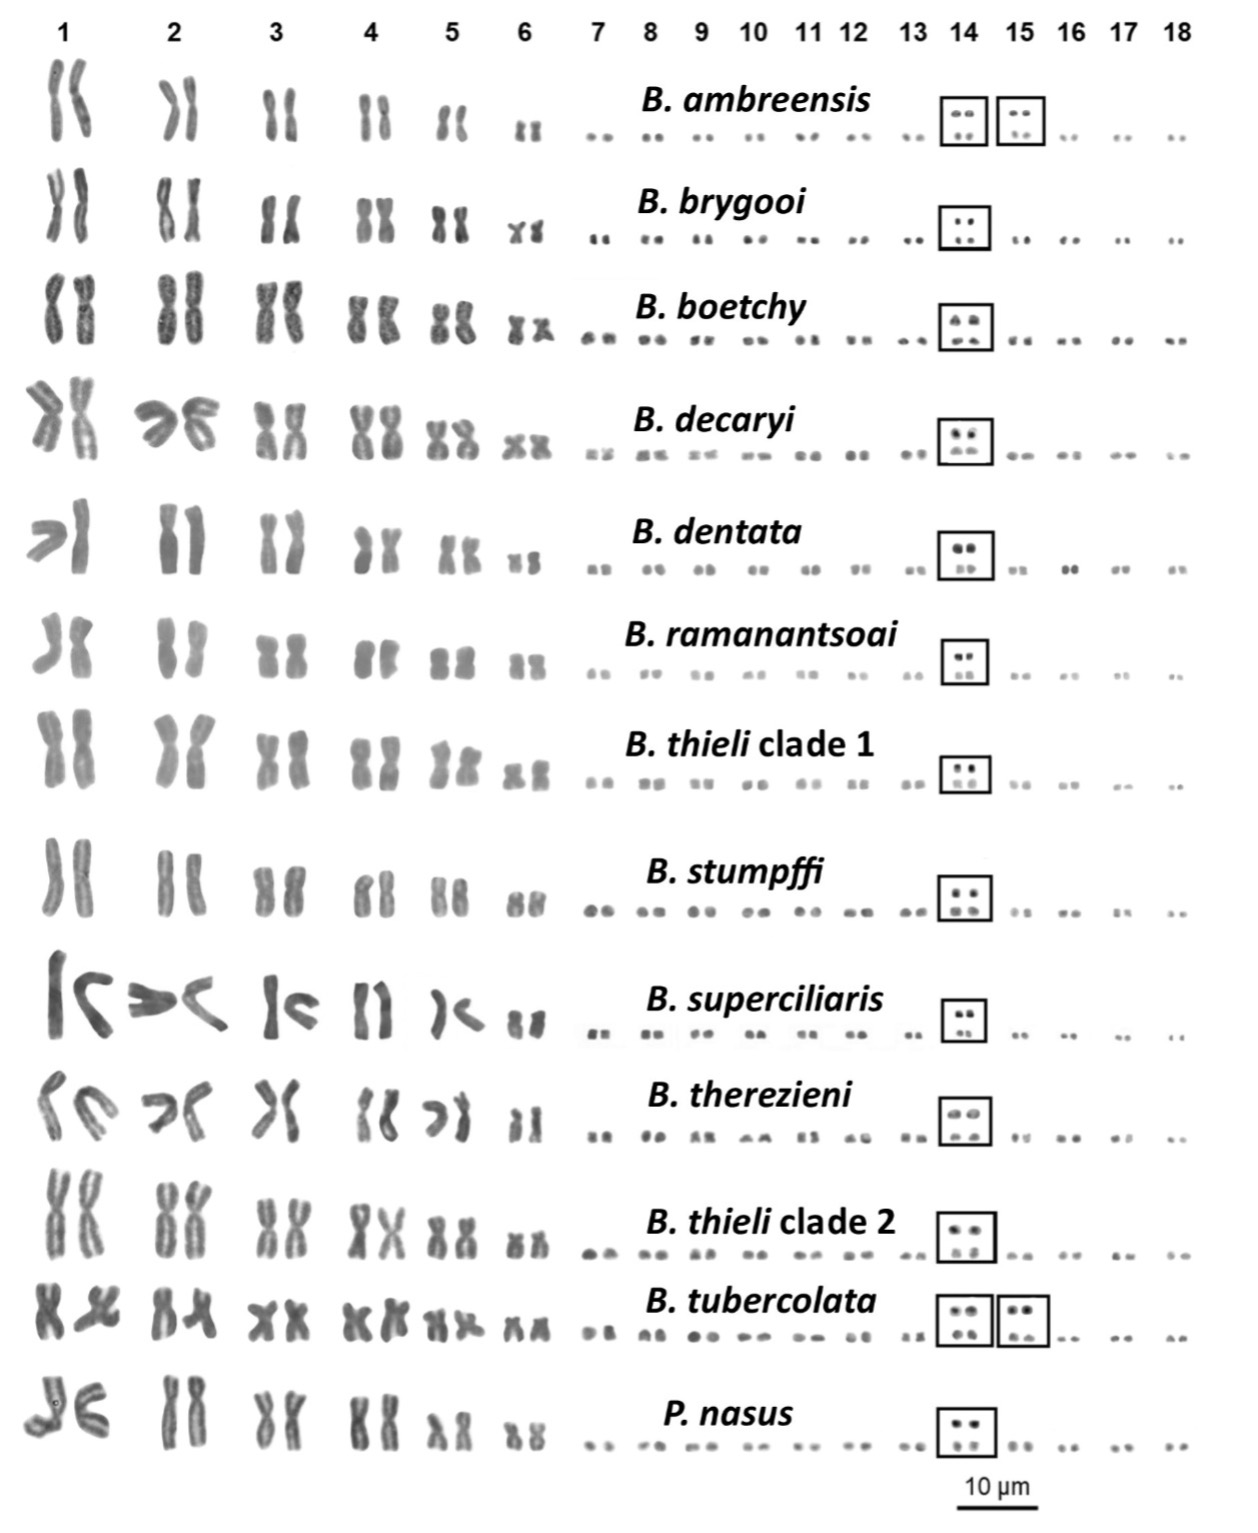
\includegraphics[width = \linewidth]{marcello-s1.jpg}
  \caption{Karyotypes of \textit{Brookesia} and \textit{Palleon} stained with Giemsa. Squares highlight the NOR-bearing chromosome pairs stained with Giemsa (left) and Ag-NOR (right).
}
  \label{fig-s1}
\end{figure}

\newpage
% marcello figure s2
\begin{figure}[h]
 \centering
  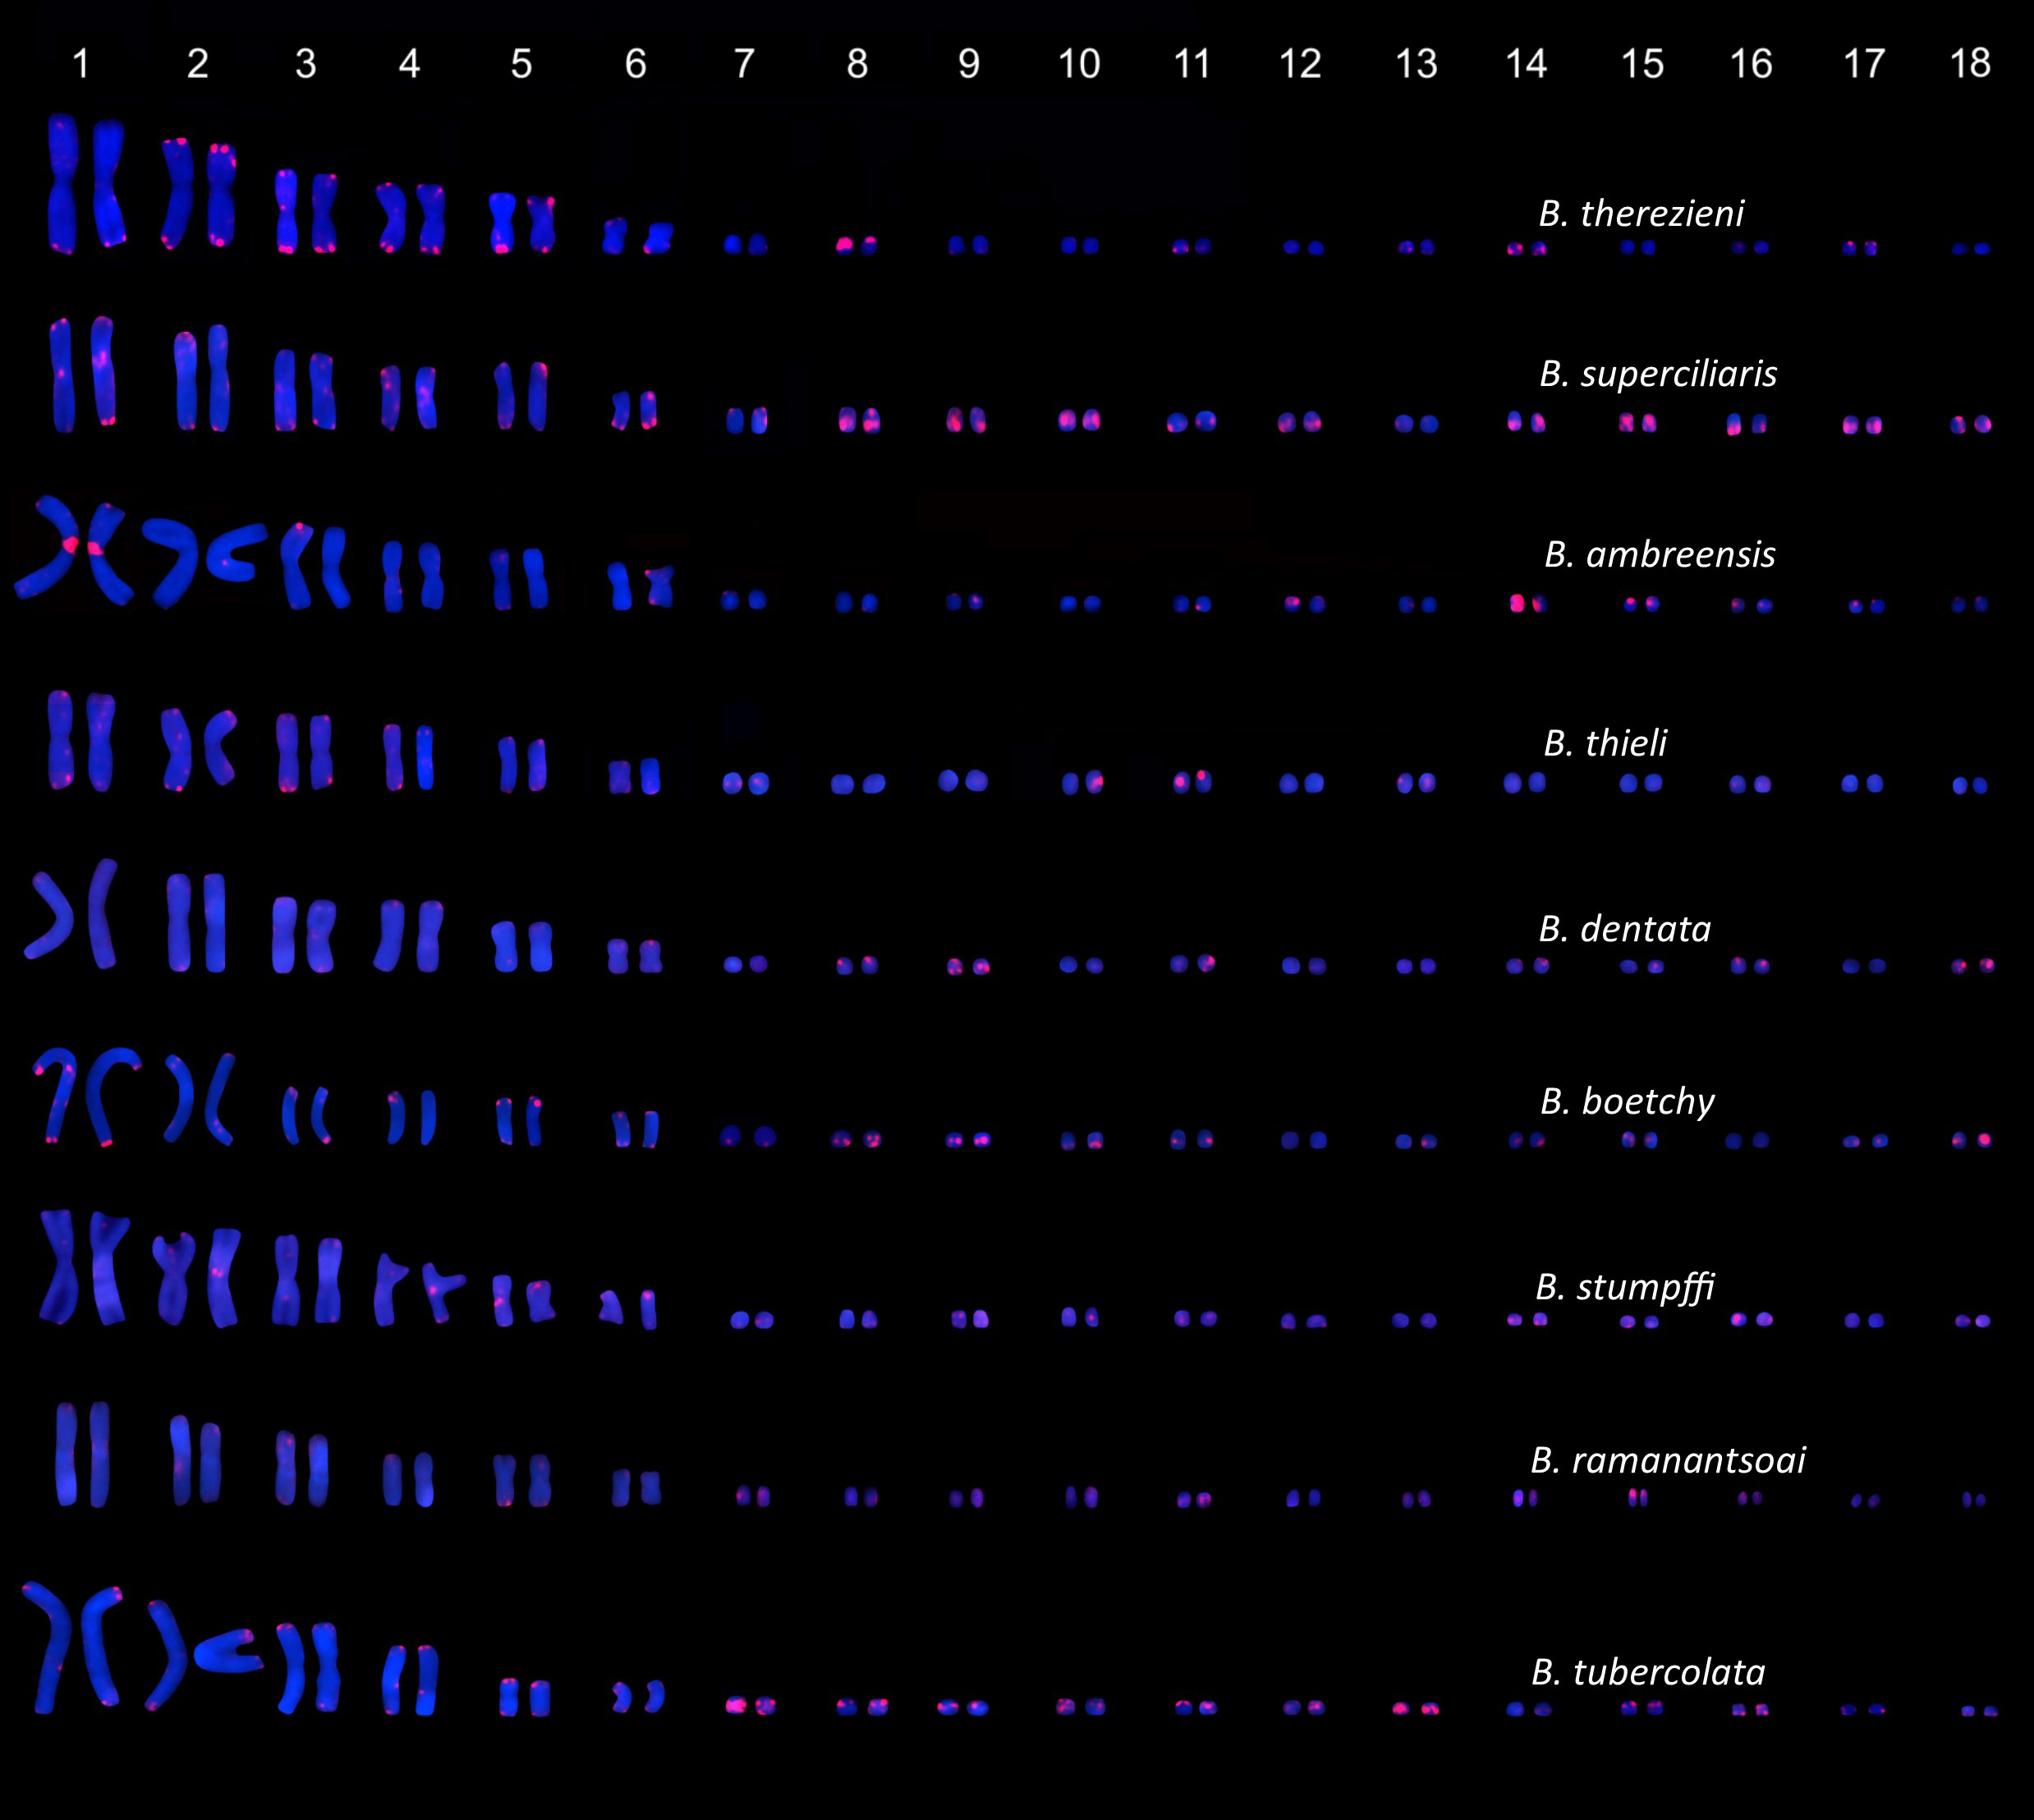
\includegraphics[width = \linewidth]{Fig2NEW.jpg}
  \caption{Karyotypes of \textit{Brookesia} and \textit{Palleon} stained with TELO-FISH.
}
  \label{fig-s2}
\end{figure}

\newpage
% marcello figure s3
\begin{figure}[h]
 \centering
  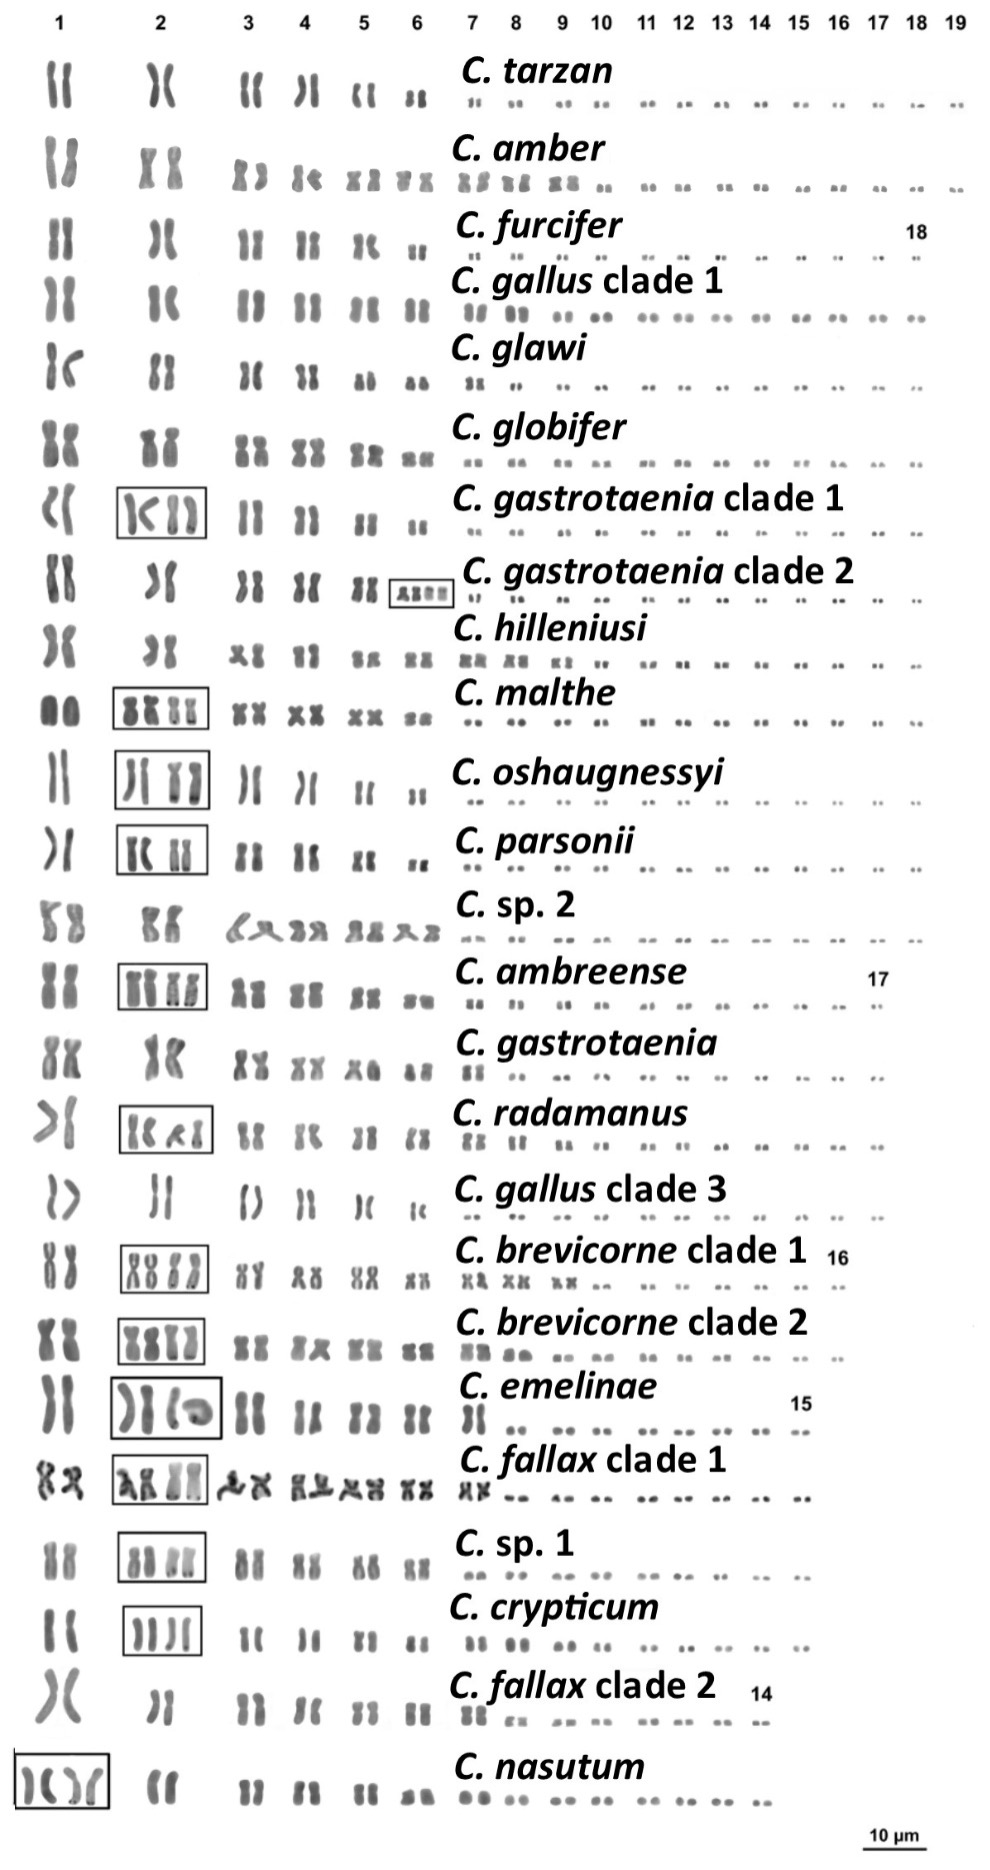
\includegraphics[width = 0.7\linewidth]{marcello-s3.jpg}
  \caption{Karyotypes of \textit{Calumma} stained with Giemsa. Squares highlight the NOR-bearing chromosome pairs stained with Giemsa (left) and Ag-NOR (right).
}
  \label{fig-s3}
\end{figure}

\newpage
% marcello fig-s4
\begin{figure}[h]
 \centering
  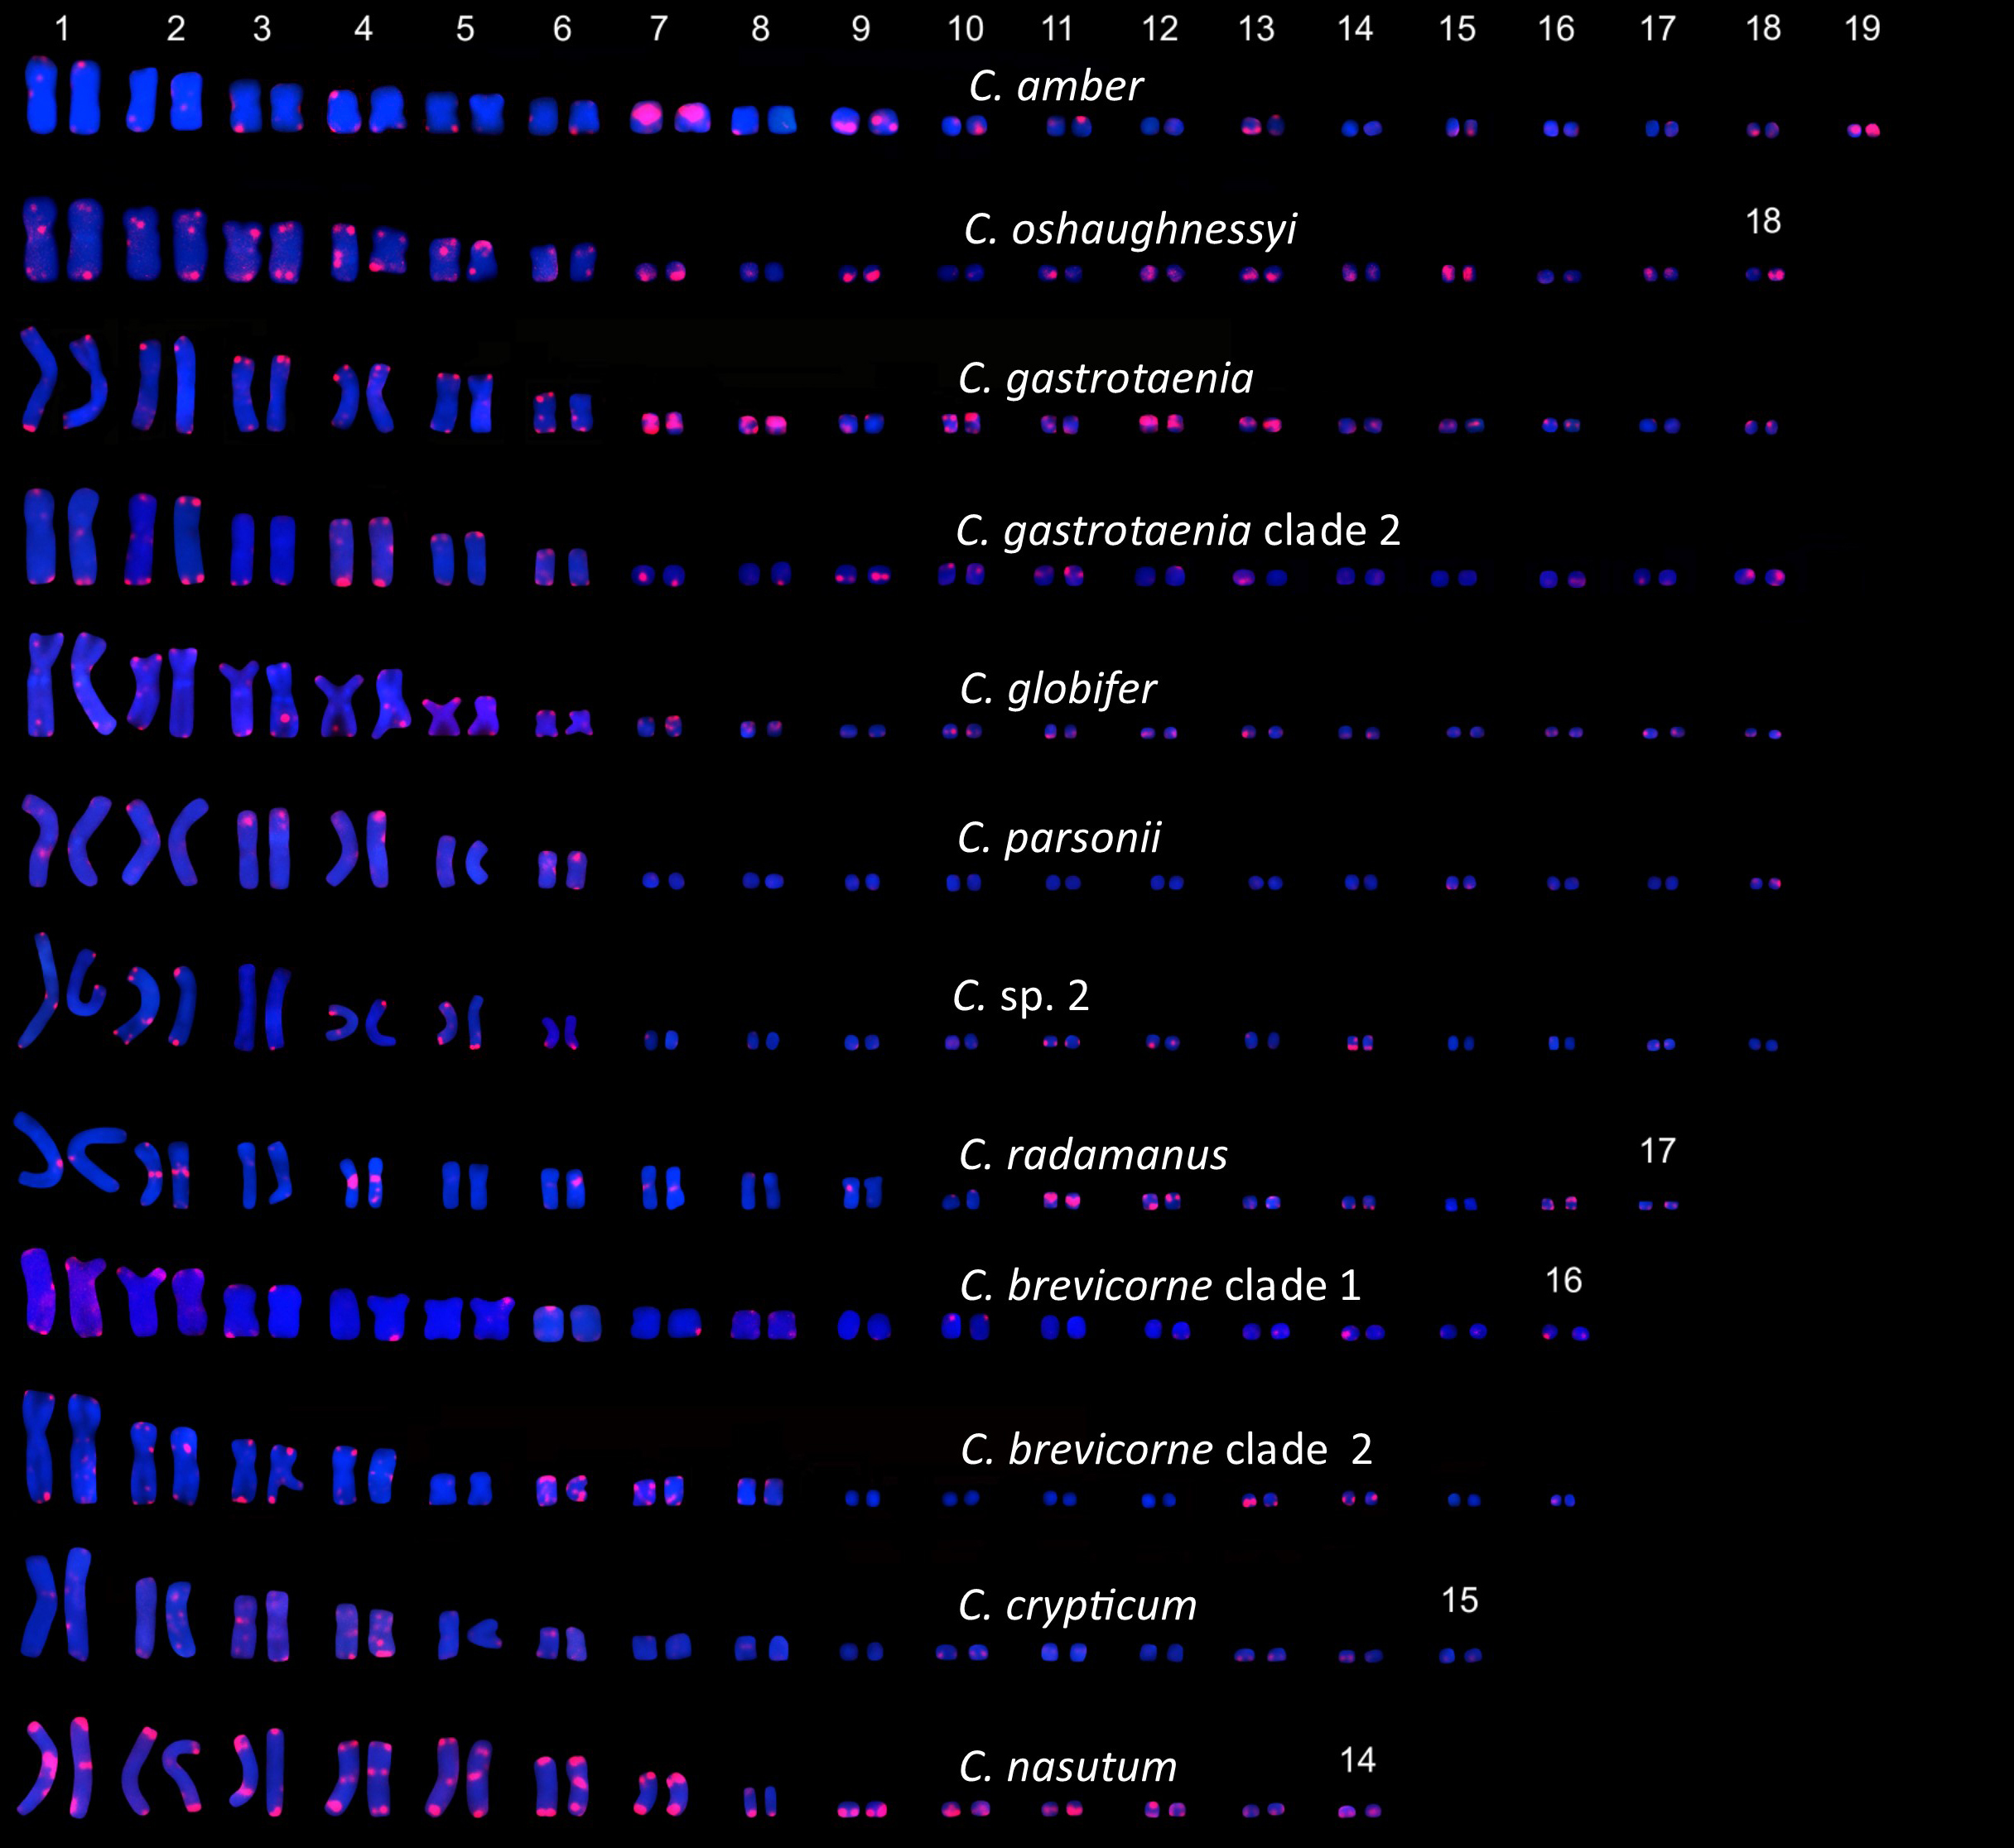
\includegraphics[width = \linewidth]{Fig4NEW.jpg}
  \caption{Karyotypes of \textit{Calumma} stained with TELO-FISH.
}
  \label{fig-s4}
\end{figure}

\newpage
% marcello figure s5
\begin{figure}[h]
 \centering
  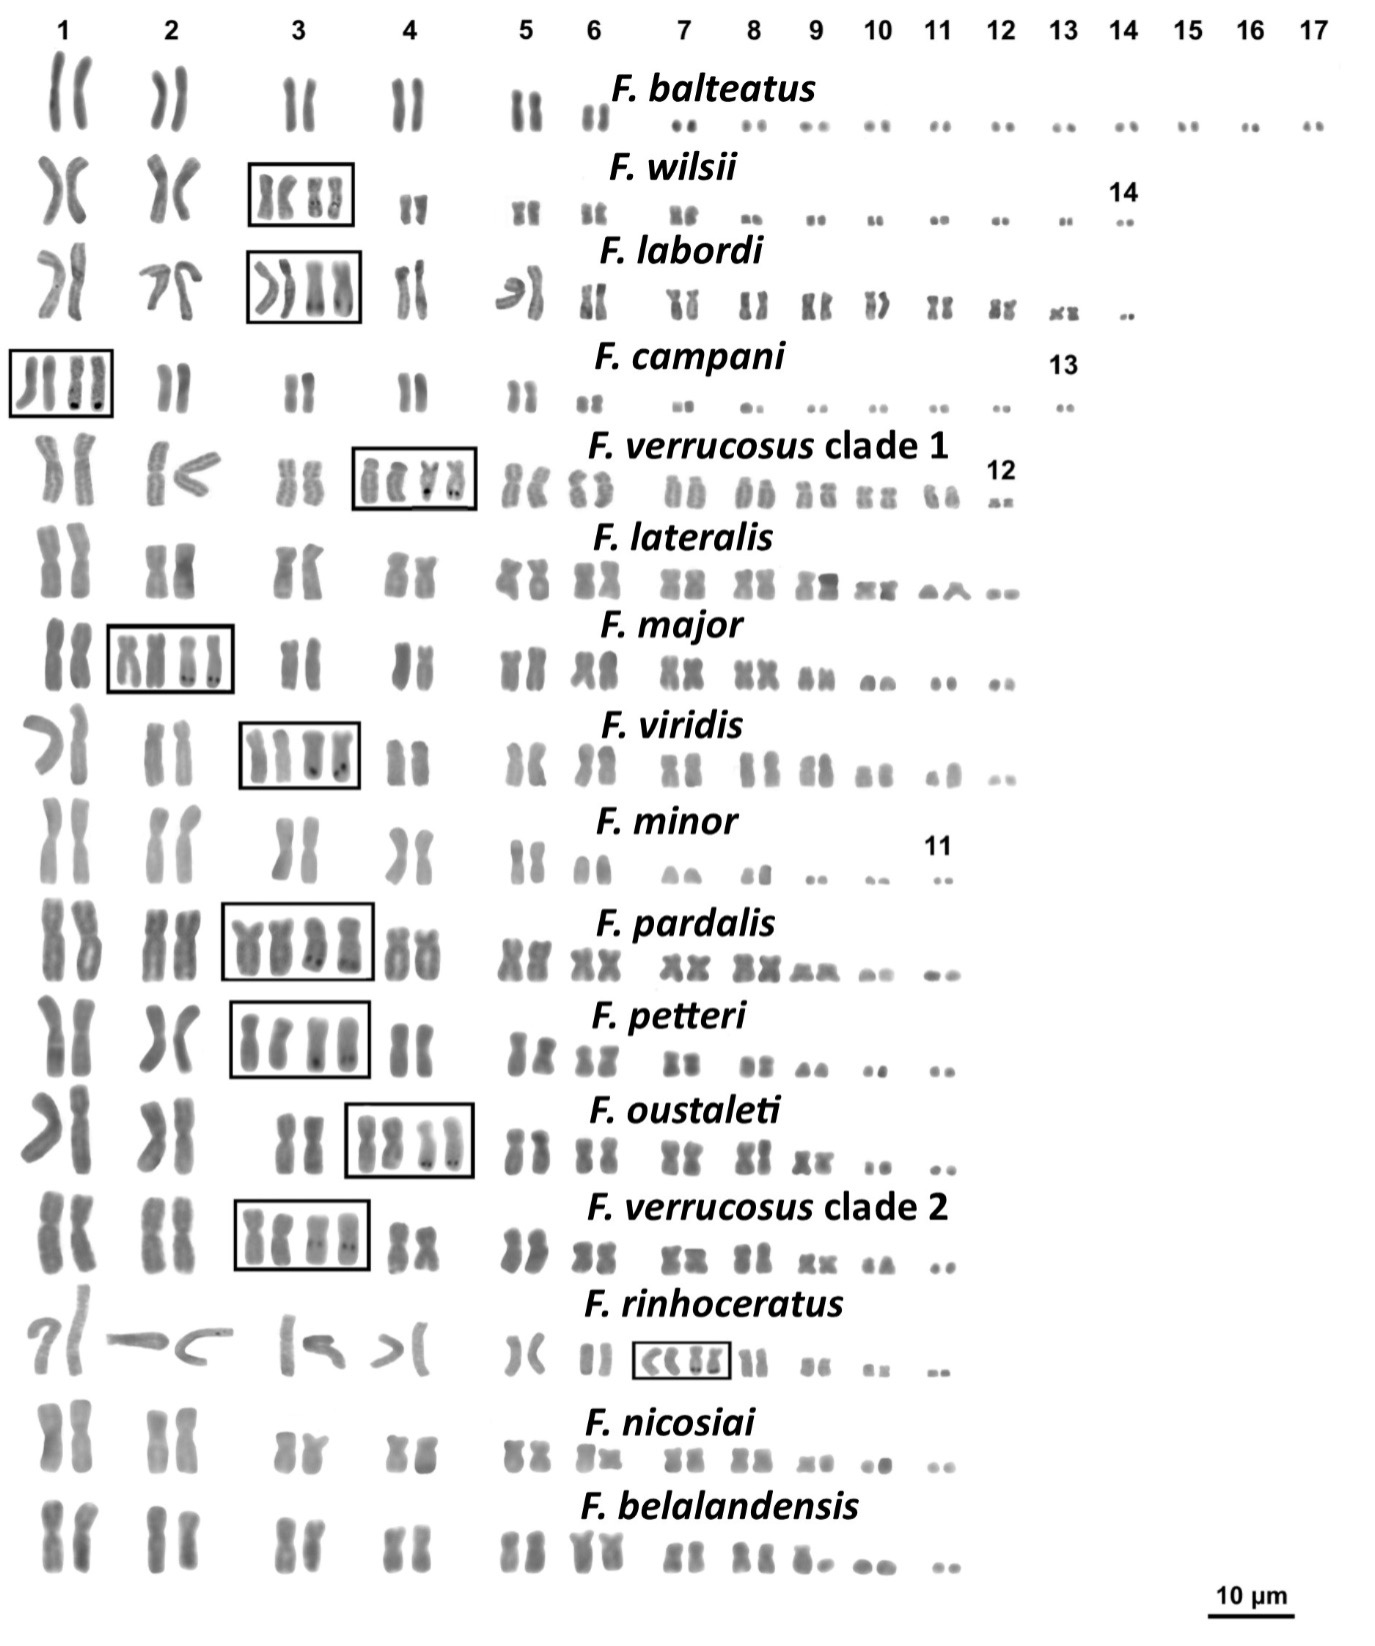
\includegraphics[width = \linewidth]{marcello-s5.jpg}
  \caption{Karyotypes of \textit{Furcifer} stained with Giemsa. Squares highlight the NOR-bearing chromosome pairs stained with Giemsa (left) and Ag-NOR (right).
}
  \label{fig-s5}
\end{figure}

\newpage
% marcello fig-s6
\begin{figure}[h]
 \centering
  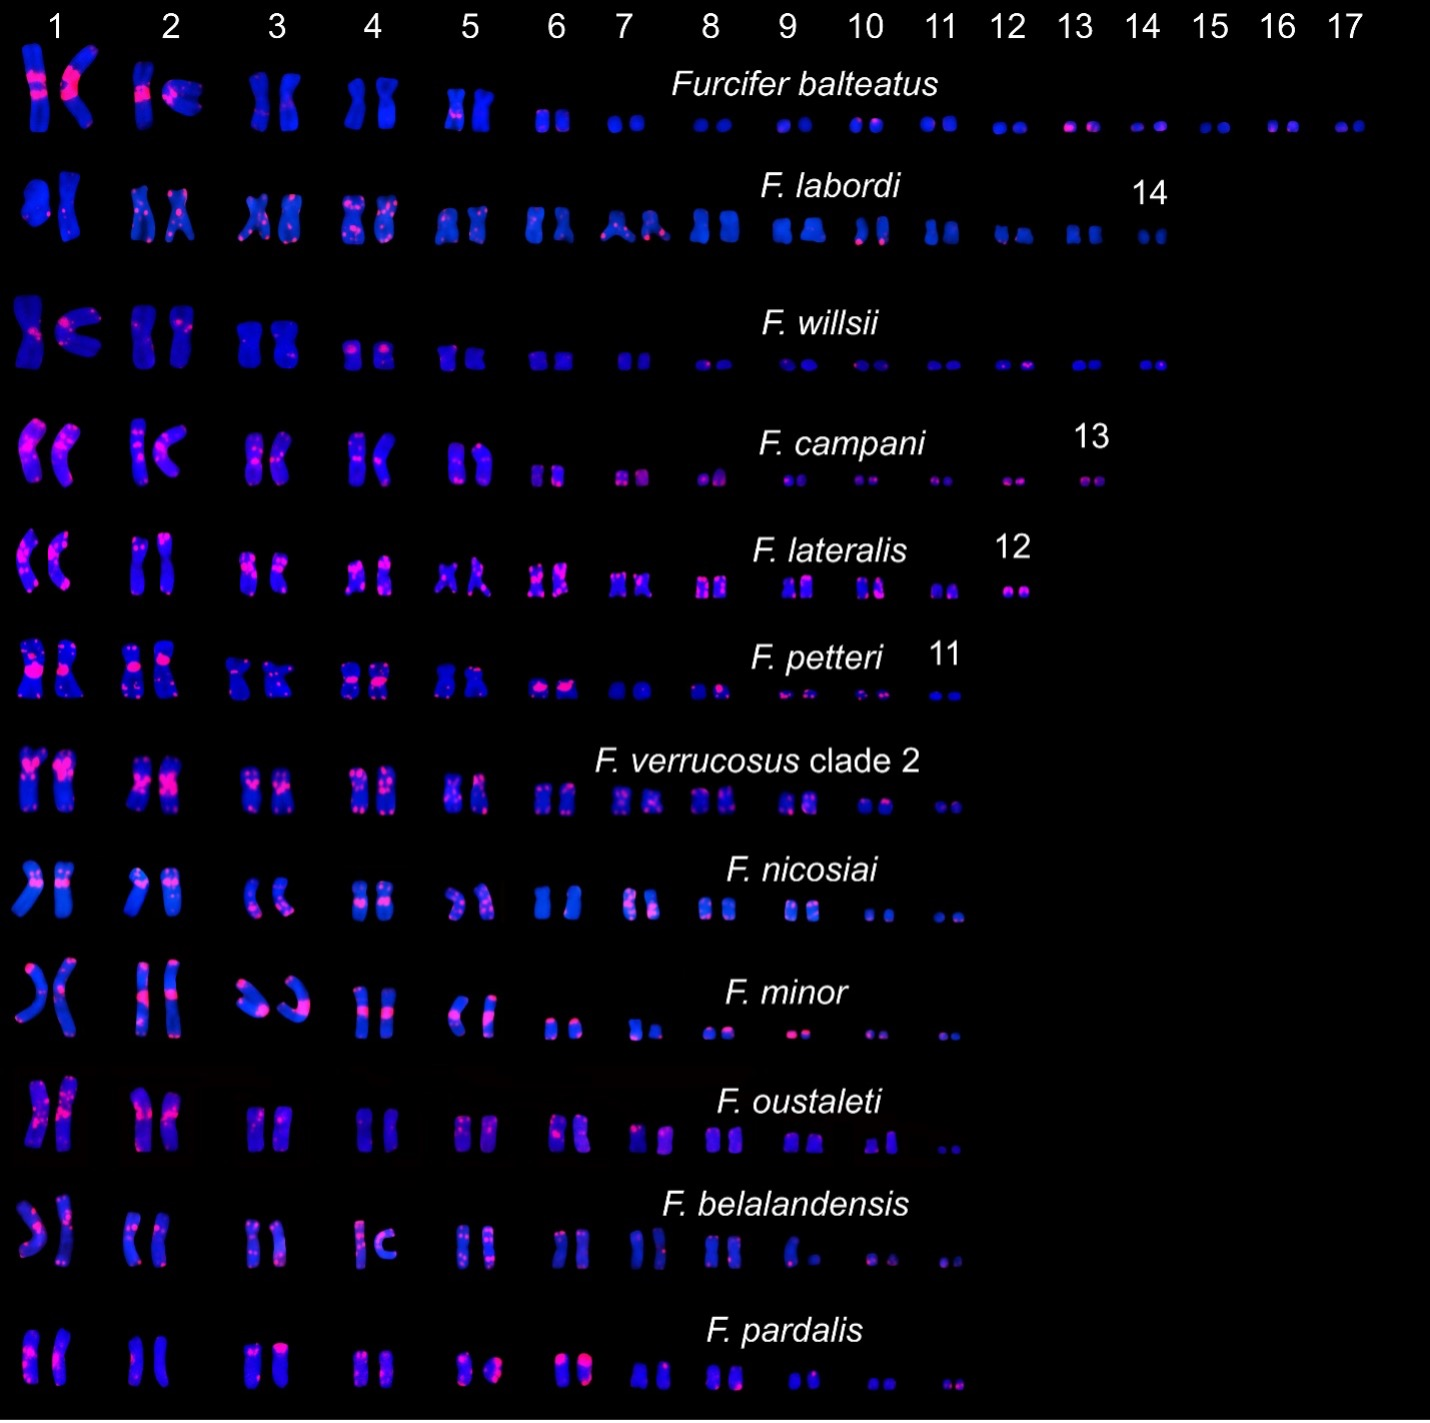
\includegraphics[width = \linewidth]{marcello-s6.jpg}
  \caption{Karyotypes of \textit{Furcifer} stained with TELO-FISH.
}
  \label{fig-s6}
\end{figure}

% figure 7
\newpage
\begin{figure}[h]
 \centering
  \includegraphics[width = \linewidth]{ChromoSSE_plot.png}
  \caption{Ancestral estimates of chromosome numbers from a ChromoSSE model, removing \textit{Rieppeleon brevicaudatus} and using n = 18 as the root frequency. Numbers at the nodes are the states with the highest posterior probability in the ChromoSSE model; numbers at the tips are the observed values. Colours represent the haploid number of chromosomes, and the size of the points at the nodes represents the posterior probability.
}
  \label{fig-best}
\end{figure}

% figure 8
\newpage
\begin{figure}[h]
 \centering
  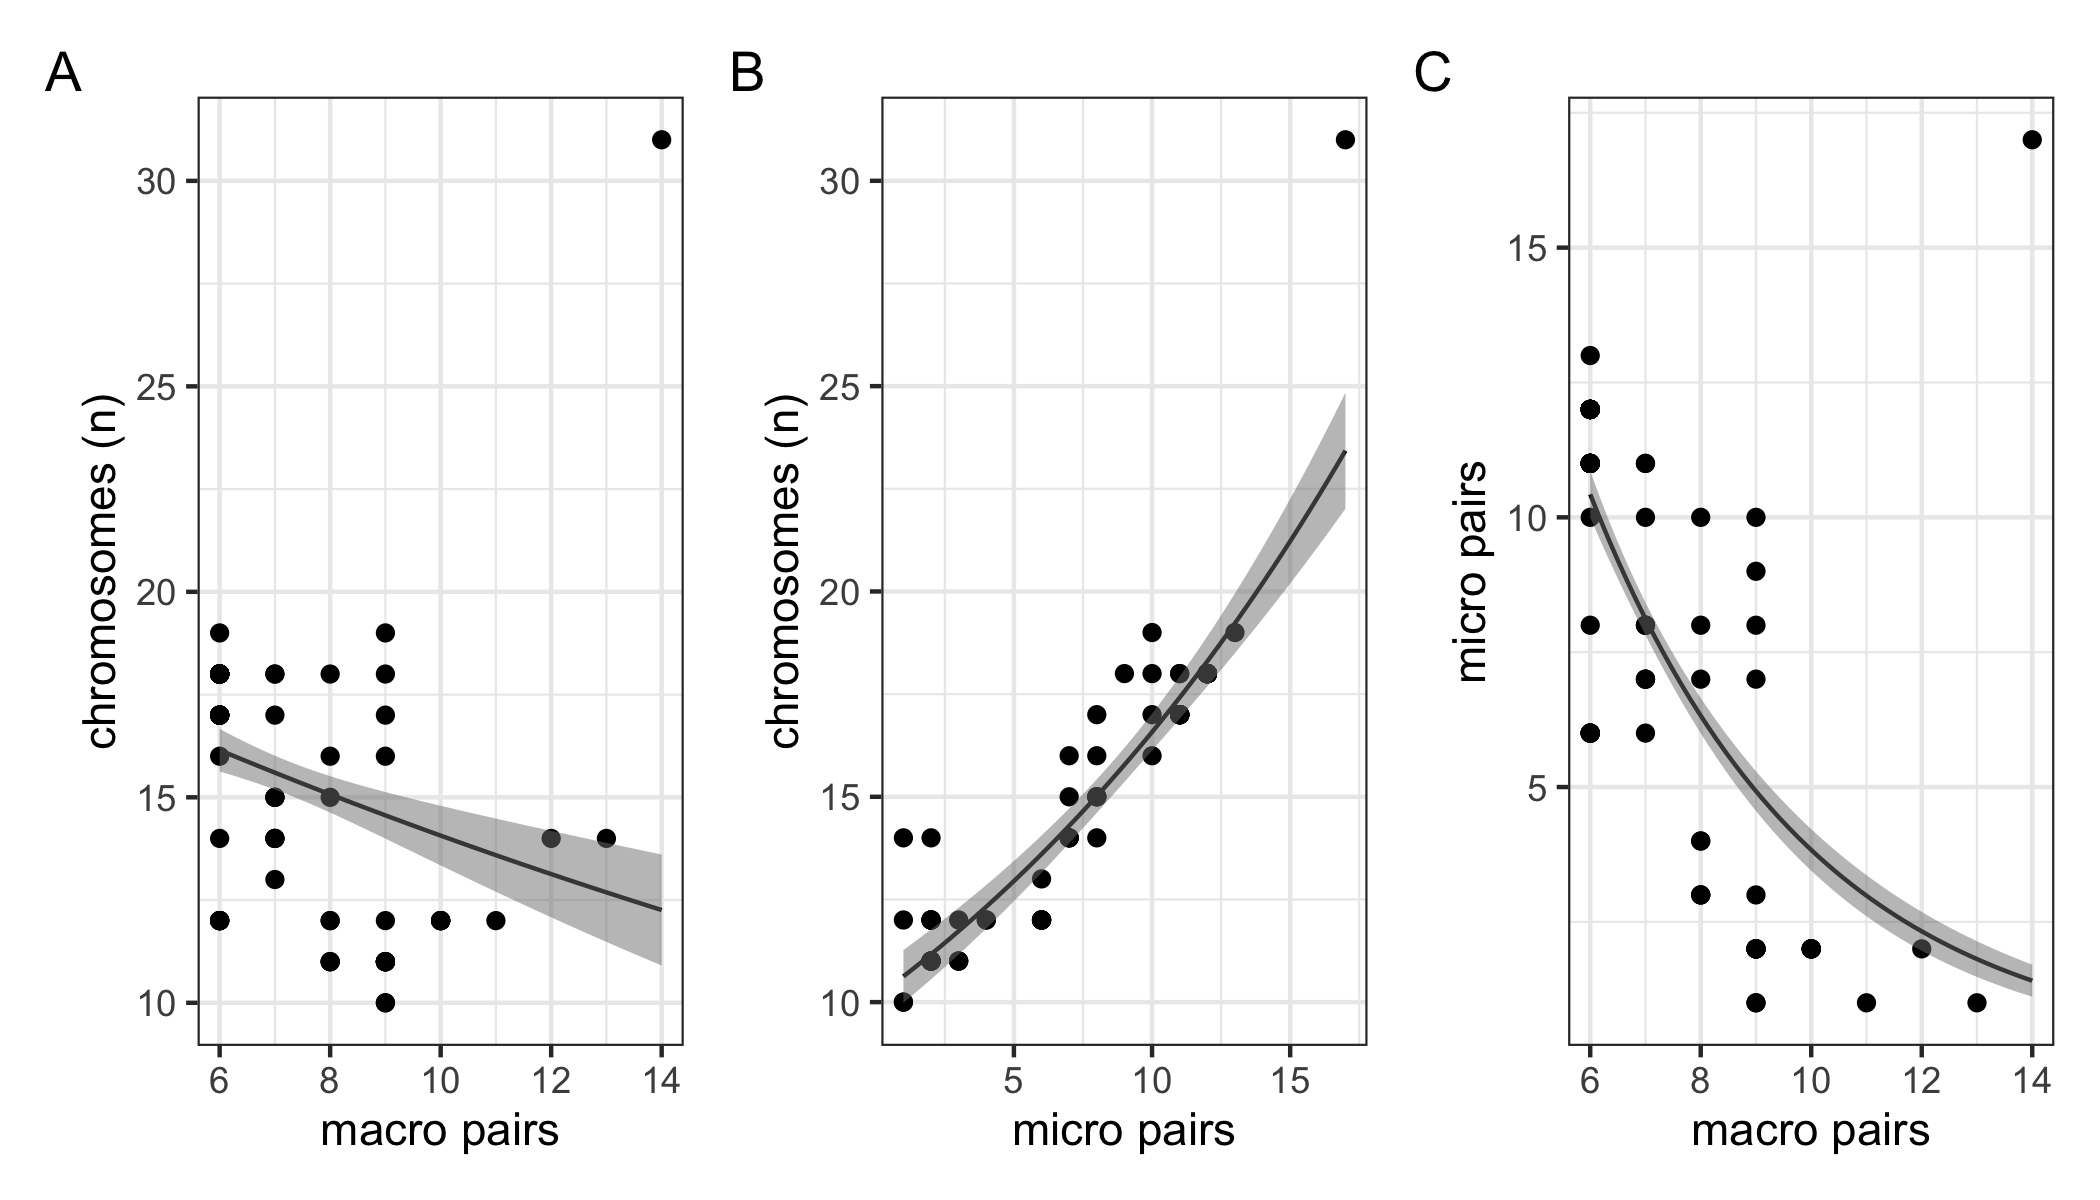
\includegraphics[width = \linewidth]{micro-macro-chromosomes.png}
  \caption{Correlations between (A) the haploid number of chromosomes (n) and numbers of macrochromosome pairs; (B) the haploid number of chromosomes (n) and numbers of microchromosome pairs; and (C) numbers of macrochromosome pairs and numbers of microchromosome pairs. Fitted lines and standard errors are the outputs from generald linear models with Poisson errors. The outlier at n = 31 is \textit{Rieppeleon brevicaudatus}.
}
  \label{fig-chroms}
\end{figure}

% figure 9
\newpage
\begin{figure}[h]
 \centering
  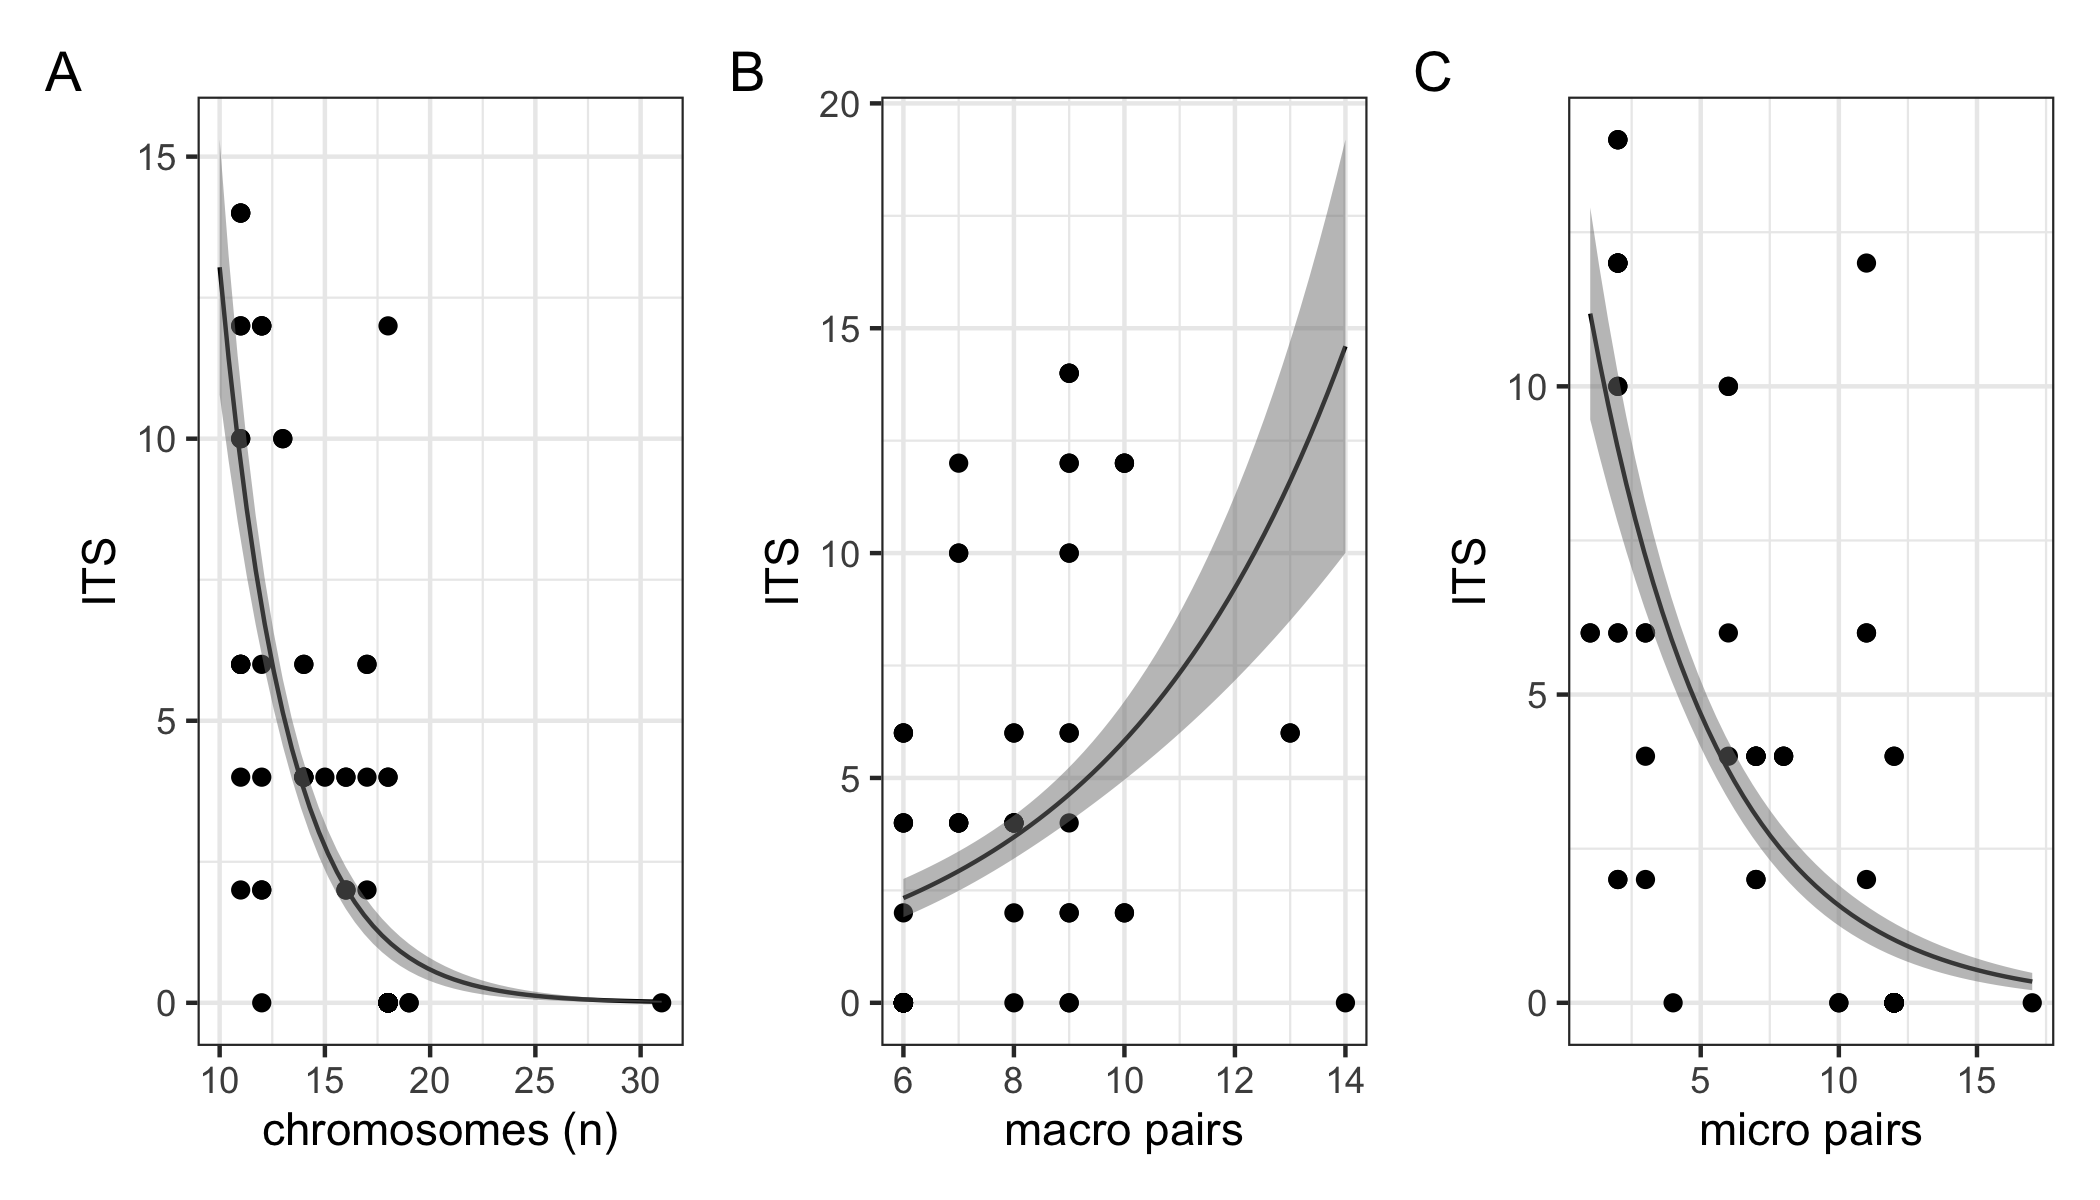
\includegraphics[width = \linewidth]{ITS-chromosomes.png}
  \caption{Correlations between (A) interstitial telomeric sequences (ITS) and the haploid number of chromosomes (n); (B) ITS and numbers of macrochromosome pairs; and (C) ITS and numbers of microchromosome pairs. Fitted lines and standard errors are the outputs from generalized linear models with quasipoisson errors. Note that we only have ITS data for 44 species.
}
  \label{fig-its}
\end{figure}

% figure 10
\newpage
\begin{figure}[h]
 \centering
  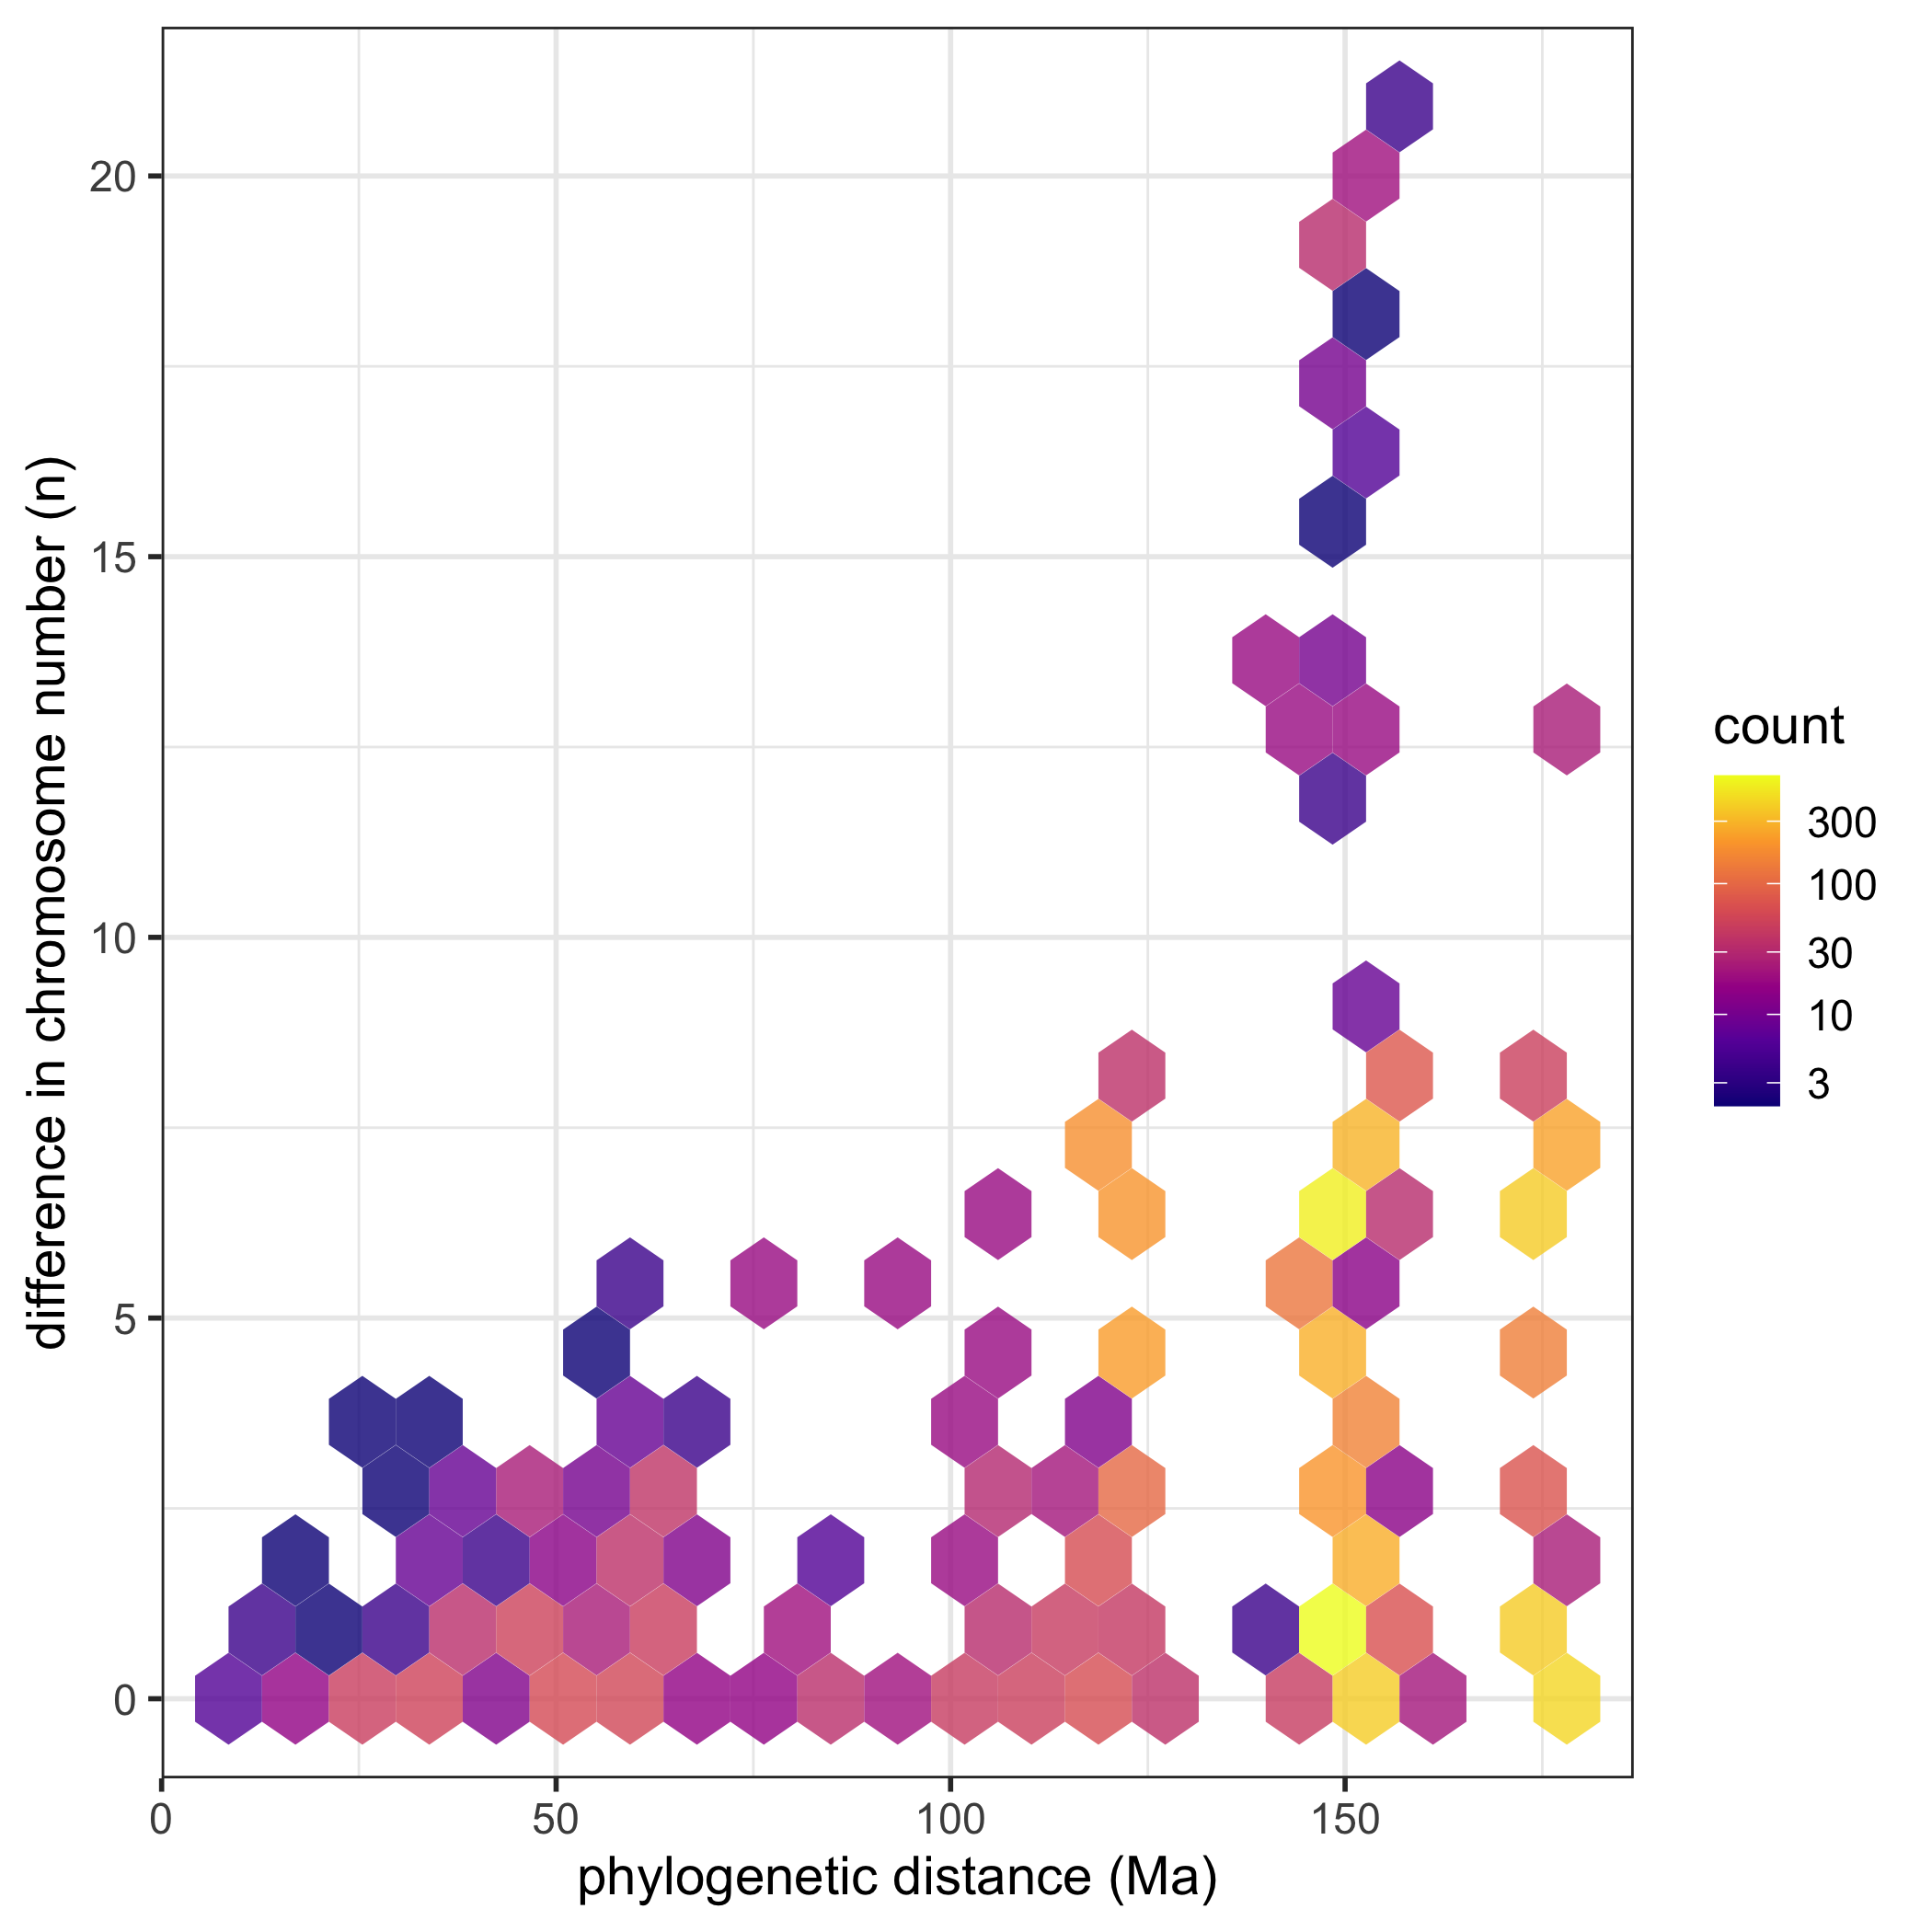
\includegraphics[width = \linewidth]{species-pairs-distances.png}
  \caption{Phylogenetic distance (in millions of years) in relation to differences in chromosome numbers (2n) for each pair of taxa in the chameleon tree. Note that the cluster of values with chromosome differences greater than 20 are comparisons of various taxa with \textit{Rieppeleon brevicaudatus} (2n = 62).}
  \label{fig-pairwise}
\end{figure}

% figure 11
\newpage
\begin{figure}[h]
 \centering
  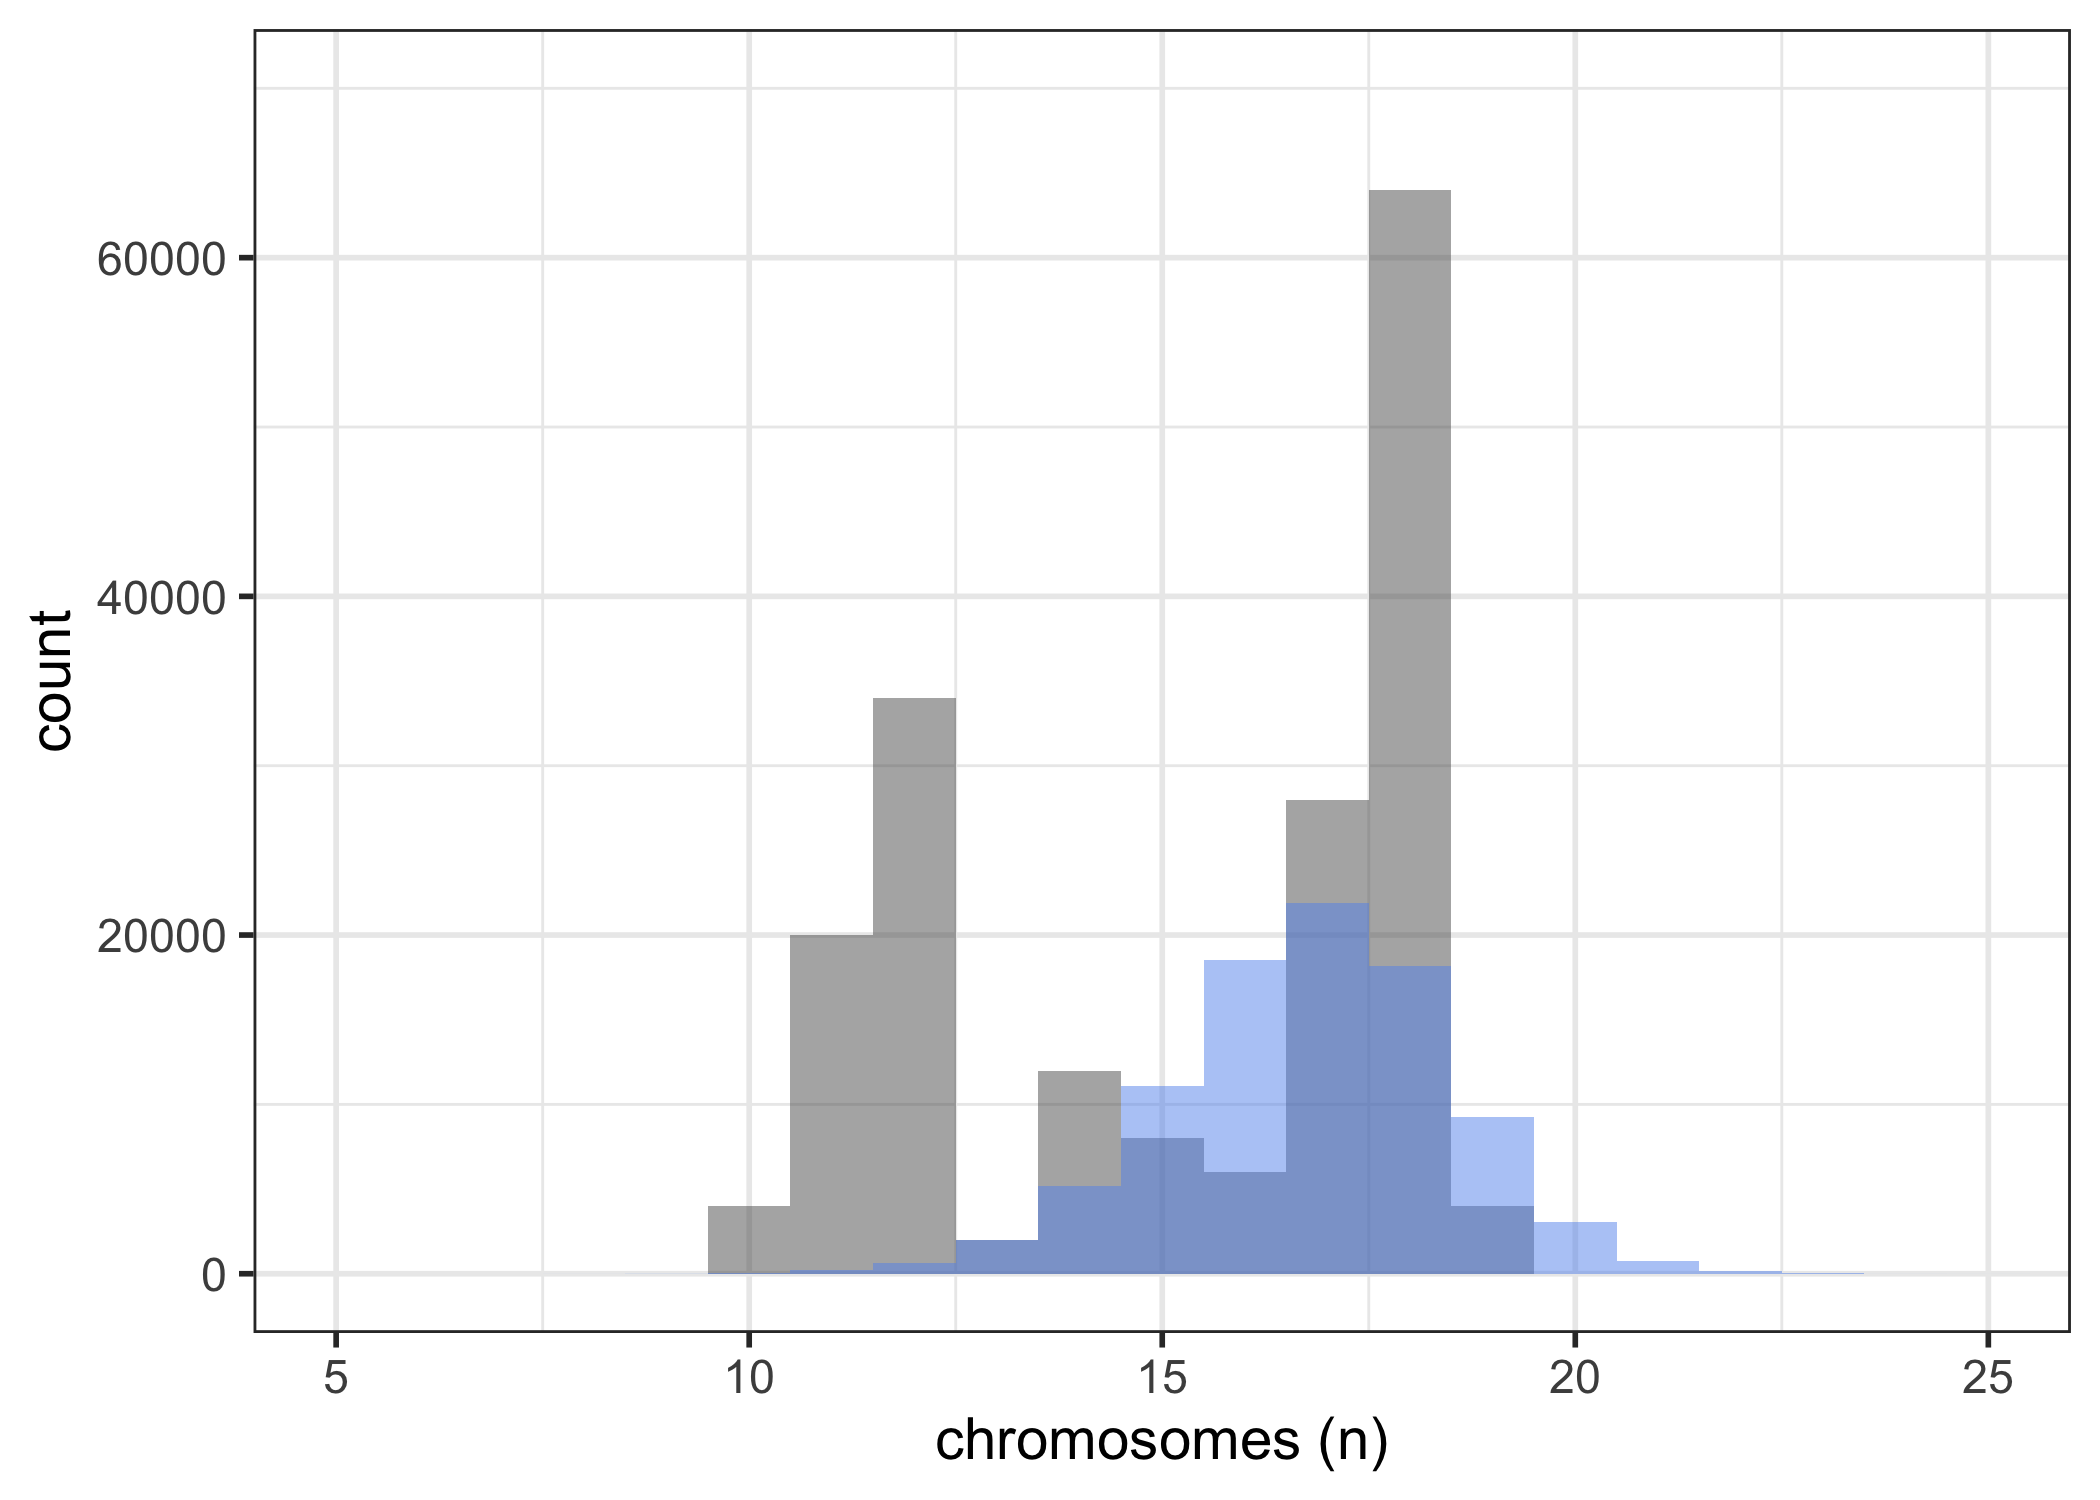
\includegraphics[width = \linewidth]{chromevol-simulations-numbers-best.png}
  \caption{Distribution of observed (grey) and predicted (blue) haploid numbers of chromosomes in chameleons, excluding \textit{Rieppeleon brevicaudatus}. Predicted values are based on 1,000 simulations using the optimized parameters taken from the best fitting model identified in the chromosome evolution analyses above (Constant Rates, removing \textit{Rieppeleon brevicaudatus}, and using n = 18 as the root frequency). Observed values were multiplied by 1,000 to aid comparisons.
}
  \label{fig-predict}
\end{figure} 

%-------------------------------------------------------------------------------
\newpage
\section{Table and figure legends}

Table 1: Results from Constant Rates and Linear Rates chromosome evolution models. root = Root frequency (see text). AIC = Akaike Information Criterion. AIC values for the best fitting model in each model set are in bold. loss = rate of chromosome loss; gain = rate of chromosome gain; lossL = linear dependency between the current haploid number and the rate of loss chromosomes; gainL = linear dependency between the current haploid number and the rate of gain chromosomes.

Figure 1: Karyotypes of \textit{Brookesia} and \textit{Palleon} stained with Giemsa. Squares highlight the NOR-bearing chromosome pairs stained with Giemsa (left) and Ag-NOR (right).

Figure 2: Karyotypes of \textit{Brookesia} and \textit{Palleon} stained with TELO-FISH.

Figure 3: Karyotypes of \textit{Calumma} stained with Giemsa. Squares highlight the NOR-bearing chromosome pairs stained with Giemsa (left) and Ag-NOR (right).

Figure 4: Karyotypes of \textit{Calumma} stained with TELO-FISH.

Figure 5: Karyotypes of \textit{Furcifer} stained with Giemsa. Squares highlight the NOR-bearing chromosome pairs stained with Giemsa (left) and Ag-NOR (right).

Figure 6: Karyotypes of \textit{Furcifer} stained with TELO-FISH.

Figure 7: Ancestral estimates of chromosome numbers from a ChromoSSE model, removing \textit{Rieppeleon brevicaudatus} and using n = 18 as the root frequency. Numbers at the nodes are the states with the highest posterior probability in the ChromoSSE model; numbers at the tips are the observed values. Colours represent the haploid number of chromosomes, and the size of the points at the nodes represents the posterior probability.

Figure 8: Correlations between (A) the haploid number of chromosomes (n) and numbers of macrochromosome pairs; (B) the haploid number of chromosomes (n) and numbers of microchromosome pairs; and (C) numbers of macrochromosome pairs and numbers of microchromosome pairs. Fitted lines and standard errors are the outputs from generalized linear models with Poisson errors. The outlier at n = 31 is \textit{Rieppeleon brevicaudatus}.

Figure 9: Correlations between (A) interstitial telomeric sequences (ITS) and the haploid number of chromosomes (n); (B) ITS and numbers of macrochromosome pairs; and (C) ITS and numbers of microchromosome pairs. Fitted lines and standard errors are the outputs from generalized linear models with quasipoisson errors. Note that we only have ITS data for 44 species. 

Figure 10: Phylogenetic distance (in millions of years) in relation to differences in chromosome numbers (2n) for each pair of taxa in the chameleon tree. Note that the cluster of values with chromosome differences greater than 20 are comparisons of various taxa with \textit{Rieppeleon brevicaudatus} (2n = 62).

Figure 11: Distribution of observed (grey) and predicted (blue) haploid numbers of chromosomes in chameleons, excluding \textit{Rieppeleon brevicaudatus}. Predicted values are based on 1,000 simulations using the optimized parameters taken from the best fitting model identified in the chromosome evolution analyses above (Constant Rates, removing \textit{Rieppeleon brevicaudatus}, and using n = 18 as the root frequency). Observed values were multiplied by 1,000 to aid comparisons.

\end{document}